\documentclass[aspectratio=169]{beamer}
\usetheme{Madrid}
\usecolortheme{default}

% Packages and settings
\usepackage[utf8]{inputenc}
\usepackage[T1]{fontenc}
\usepackage{amsmath,amssymb,amsfonts}
\usepackage{graphicx}
\usepackage{booktabs}
\usepackage{multirow}
\usepackage{tikz}
\usepackage{pgfplots}
\usepackage{xcolor}
\usepackage{url}
\usepackage{amssymb} % for checkmark symbol

% PGFPlots compatibility
\pgfplotsset{compat=1.18}

% Custom colors
\definecolor{zjutblue}{RGB}{0,82,155}
\definecolor{zjutred}{RGB}{220,20,60}
\definecolor{zjutgreen}{RGB}{34,139,34}

% Theme colors
\setbeamercolor{structure}{fg=zjutblue}
\setbeamercolor{frametitle}{bg=zjutblue,fg=white}
% \setbeamercolor{title}{fg=zjutblue}

% Title information
% \title[GRCR-Net]{GRCR-Net: A Complex Residual Network with GPR Denoising\\[0.3cm]and Rotational Augmentation for Automatic Modulation Classification}
% \subtitle{A Breakthrough Approach for AMC}
\title[GRCR-Net]{GRCR-Net: A Complex Residual Network with GPR Denoising\\and Rotational Augmentation for Automatic Modulation Classification\\[0.3cm]}
\subtitle{A Breakthrough Approach for AMC}
\author[Junkai Li]{Junkai Li}
\institute[ZJUT]{College of Information Engineering\\Zhejiang University of Technology}
\date{July 5, 2025}

% Begin document
\begin{document}

% --- FIX START ---
% The original code manually created a title page using beamercolorbox.
% The standard and recommended way to generate a title page in Beamer
% is to use the \titlepage command within a frame. This ensures that
% the theme's design is applied correctly and PDF metadata (like the
% document title) is properly set.
\begin{frame}
    \titlepage
\end{frame}
% --- FIX END ---

% Table of contents
\begin{frame}{Outline}
\tableofcontents
\end{frame}

% Section 1: Background and Challenges
\section{Background and Challenges}

\begin{frame}{The Importance of Automatic Modulation Classification}
\begin{columns}
\begin{column}{0.6\textwidth}
\textbf{Critical Applications:}
\begin{itemize}
\item \textbf{Cognitive Radio}: Dynamic spectrum sensing and management
\item \textbf{Spectrum Monitoring}: Radio environment situational awareness
\item \textbf{Military Communications}: Electronic warfare and signal intelligence
\item \textbf{5G/6G Networks}: Intelligent signal processing
\end{itemize}

\vspace{0.5cm}
\textbf{Key Challenge:}
\begin{itemize}
\item Accurate classification under low Signal-to-Noise Ratio (SNR)
\item Preserving I/Q signal phase information
\item Robust performance in complex electromagnetic environments
\end{itemize}
\end{column}
\begin{column}{0.4\textwidth}
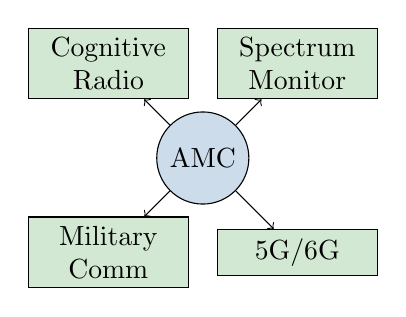
\begin{tikzpicture}[scale=0.8]
\node[draw,circle,fill=zjutblue!20] (amc) at (0,0) {AMC};
\node[draw,rectangle,fill=zjutgreen!20,text width=1.8cm,align=center] (cr) at (-1.5,1.5) {Cognitive\\Radio};
\node[draw,rectangle,fill=zjutgreen!20,text width=1.8cm,align=center] (sm) at (1.5,1.5) {Spectrum\\Monitor};
\node[draw,rectangle,fill=zjutgreen!20,text width=1.8cm,align=center] (mc) at (-1.5,-1.5) {Military\\Comm};
\node[draw,rectangle,fill=zjutgreen!20,text width=1.8cm,align=center] (ic) at (1.5,-1.5) {5G/6G};
\draw[->] (amc) -- (cr);
\draw[->] (amc) -- (sm);
\draw[->] (amc) -- (mc);
\draw[->] (amc) -- (ic);
\end{tikzpicture}
\end{column}
\end{columns}
\end{frame}

\begin{frame}{Core Challenge: Performance Degradation in Low SNR}
\begin{columns}
\begin{column}{0.5\textwidth}
\textbf{Limitations of Existing Methods:}
\begin{itemize}
\item Likelihood-based methods: High computational complexity
\item Feature-based methods: Rely on expert knowledge
\item Deep learning methods: Severe performance drop in low SNR
\end{itemize}

\vspace{0.5cm}
\textbf{Critical Issues:}
\begin{itemize}
\item Noise severely affects signal quality
\item Loss of I/Q signal phase information
\item Data imbalance and poor generalization
\end{itemize}
\end{column}
\begin{column}{0.5\textwidth}
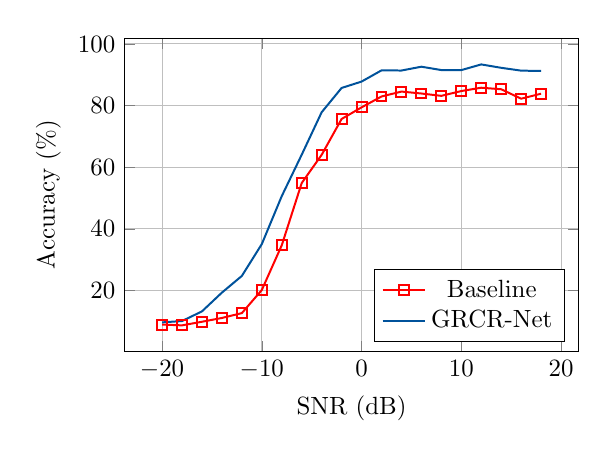
\begin{tikzpicture}[scale=0.9]
\begin{axis}[
    xlabel={SNR (dB)},
    ylabel={Accuracy (\%)},
    grid=major,
    legend pos=south east,
    width=8cm,
    height=6cm
]
\addplot[color=red,mark=square,thick,mark size=2pt] coordinates {
    (-20,8.93) (-18,8.68) (-16,9.85) (-14,11.08) (-12,12.65) (-10,20.15)
    (-8,34.66) (-6,54.86) (-4,64.02) (-2,75.66) (0,79.43) (2,82.96)
    (4,84.56) (6,83.93) (8,83.17) (10,84.73) (12,85.81) (14,85.31)
    (16,82.25) (18,83.87)
};
\addplot[color=zjutblue,mark=circle,thick,mark size=2pt] coordinates {
    (-20,9.65) (-18,10.08) (-16,13.21) (-14,19.31) (-12,24.72) (-10,35.05)
    (-8,50.62) (-6,64.05) (-4,77.84) (-2,85.73) (0,87.80) (2,91.44)
    (4,91.39) (6,92.63) (8,91.54) (10,91.53) (12,93.37) (14,92.27)
    (16,91.35) (18,91.25)
};
% \legend{Traditional,GRCR-Net}
\legend{Baseline,GRCR-Net}
\end{axis}
\end{tikzpicture}
\end{column}
\end{columns}
\end{frame}


\begin{frame}{Power Analysis: Visual Understanding}
\begin{center}
\textcolor{zjutblue}{\Large \textbf{Understanding Power Relationships}}
\end{center}

\vspace{0.3cm}
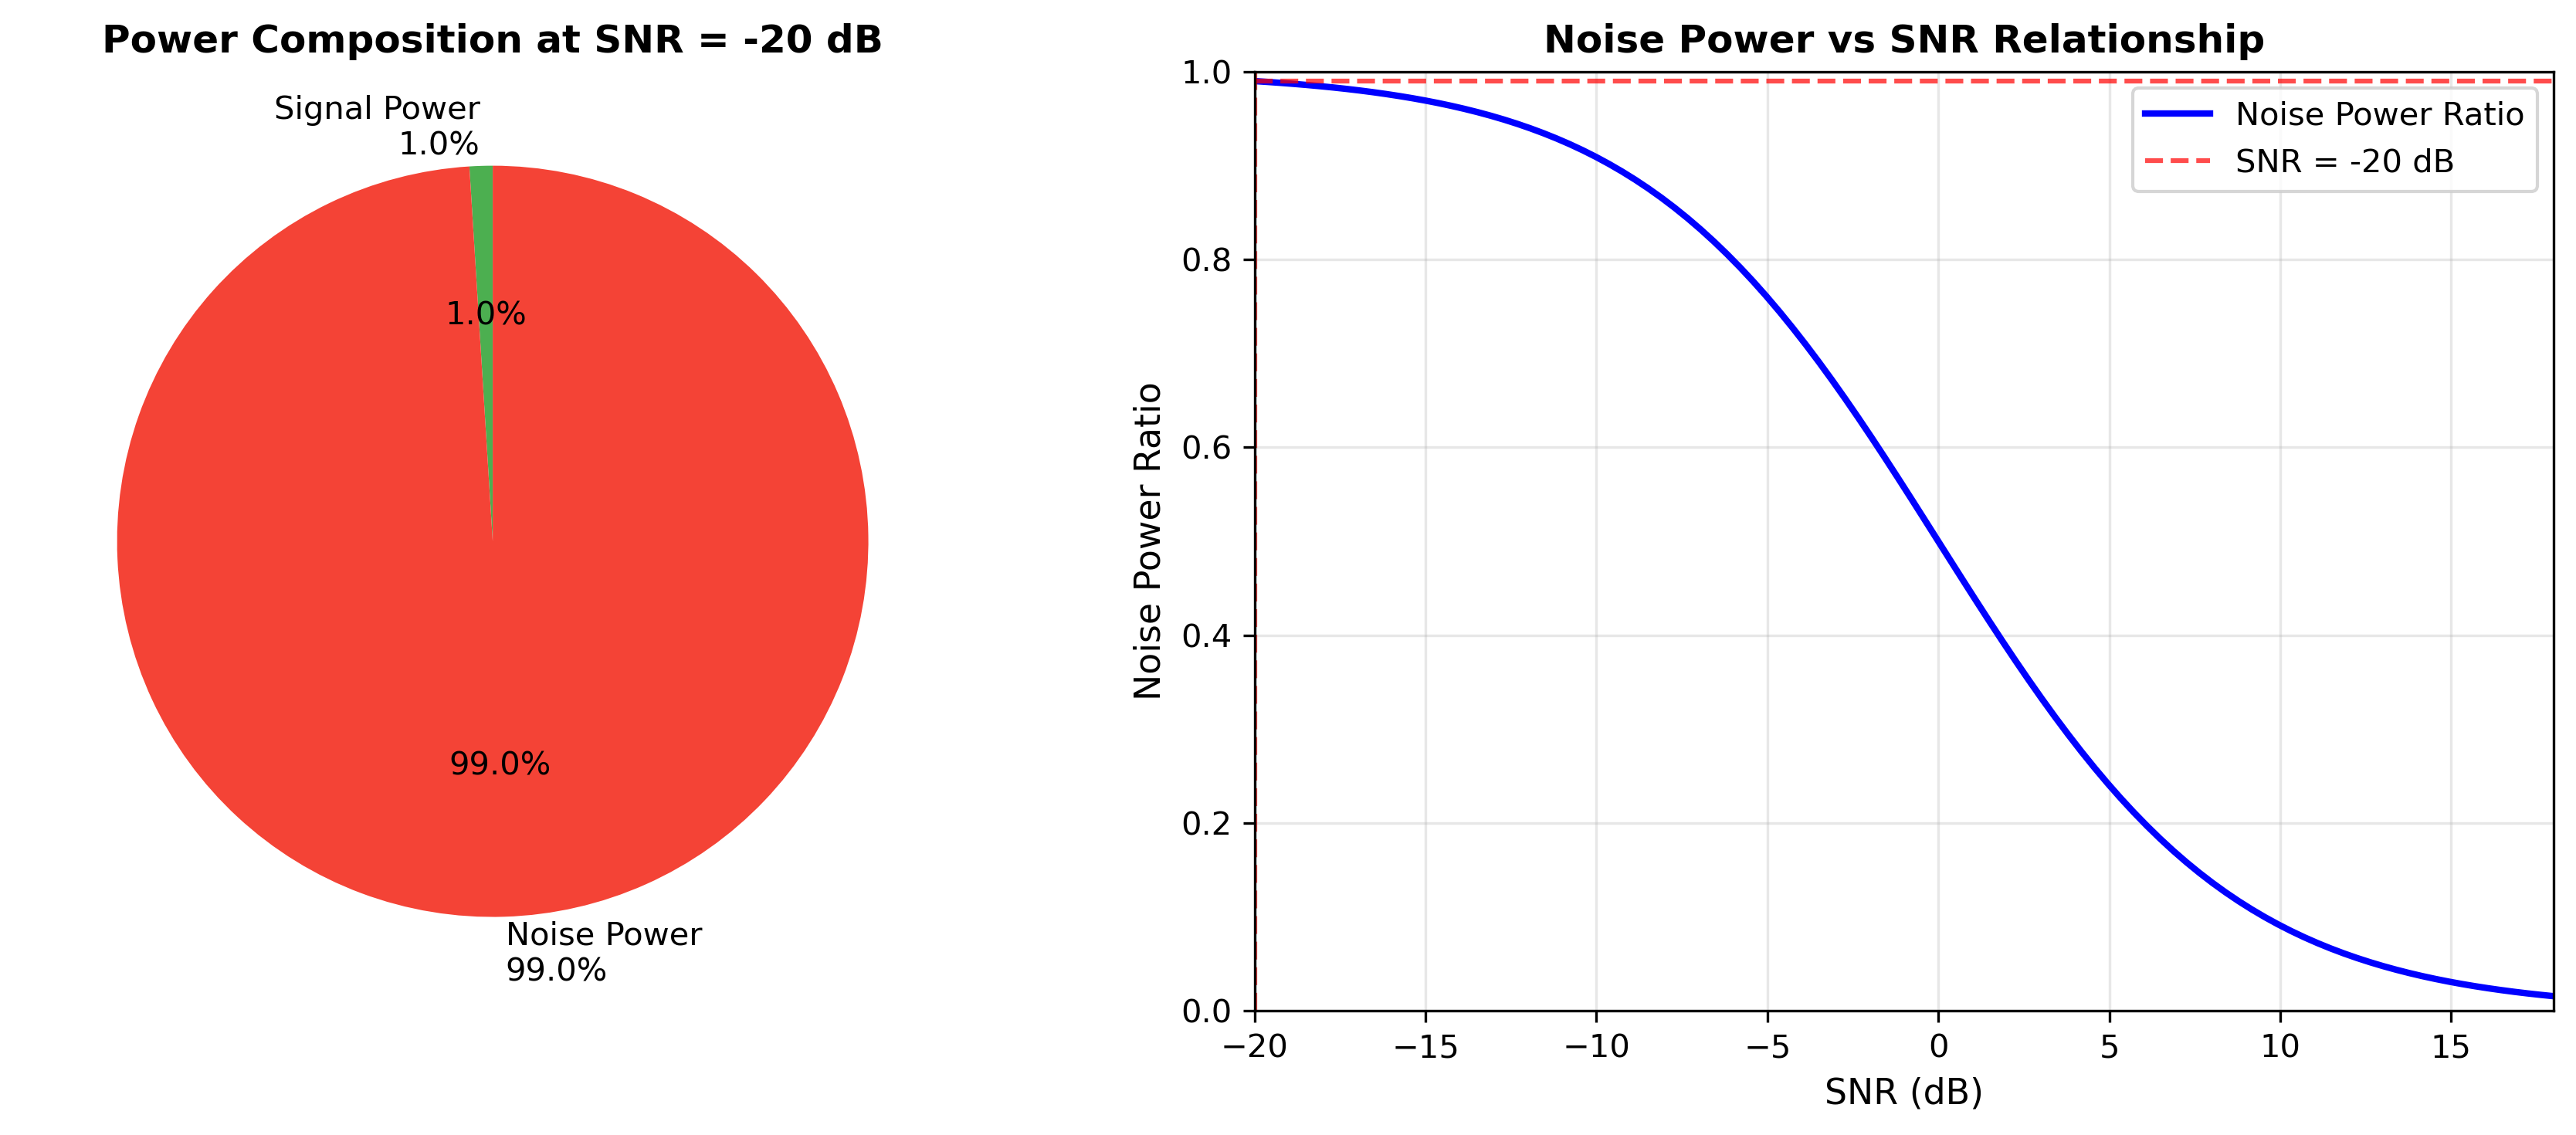
\includegraphics[width=\textwidth]{figure/power_analysis.png}

\vspace{0.3cm}
\begin{center}
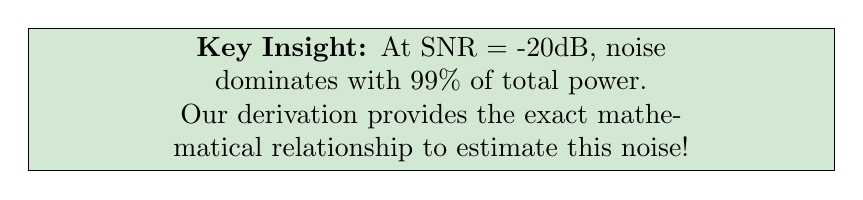
\begin{tikzpicture}[scale=0.8]
\node[draw,rectangle,fill=zjutgreen!20,text width=10cm,align=center] at (0,0) {
\textbf{Key Insight:} At SNR = -20dB, noise dominates with 99\% of total power. \\
Our derivation provides the exact mathematical relationship to estimate this noise!
};
\end{tikzpicture}
\end{center}
\end{frame}



\begin{frame}{The Challenge: Extreme Noise Conditions}
\begin{center}
\textcolor{zjutred}{\Large \textbf{SNR = -20dB: Signal Power Only 1\%, Noise 99\%}}
\end{center}

\vspace{0.5cm}
\begin{columns}
\begin{column}{0.6\textwidth}
\textbf{Extreme Low SNR Challenge:}
\begin{itemize}
\item At SNR = -20dB: $P_{\text{signal}} = 1\%$, $P_{\text{noise}} = 99\%$
\item Previous SOTA methods: only $\sim$60\% accuracy
\item Massive noise severely degrades classification
\item Traditional denoising methods fail
\end{itemize}

\vspace{0.3cm}
\textbf{Our Solution: Adaptive GPR Denoising}
\begin{itemize}
\item Model signal as Gaussian Process
\item Assume Additive White Gaussian Noise (AWGN)
\item Derive noise power from signal statistics
\item Adaptive scale parameters for different SNRs
\end{itemize}
\end{column}
\begin{column}{0.4\textwidth}
\begin{center}
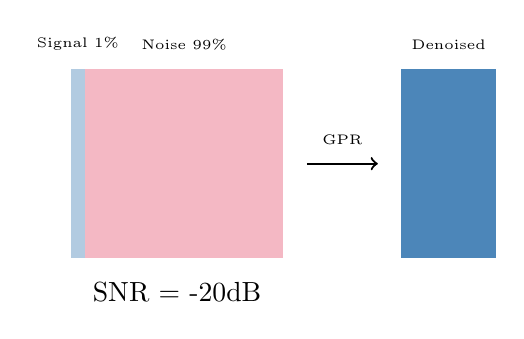
\begin{tikzpicture}[scale=0.6]
% Signal vs Noise visualization
\fill[zjutblue!30] (0,0) rectangle (0.3,4);
\fill[zjutred!30] (0.3,0) rectangle (4.5,4);

\node[anchor=south] at (0.15,4.2) {\tiny Signal 1\%};
\node[anchor=south] at (2.4,4.2) {\tiny Noise 99\%};

\node[anchor=north] at (2.25,-0.3) {SNR = -20dB};

% Arrow showing improvement
\draw[thick,->] (5,2) -- (6.5,2);
\node at (5.75,2.5) {\tiny GPR};

% After denoising
\fill[zjutblue!70] (7,0) rectangle (9,4);
\node[anchor=south] at (8,4.2) {\tiny Denoised};
\end{tikzpicture}
\end{center}
\end{column}
\end{columns}
\end{frame}

\begin{frame}{Why Tackle the Impossible? The Value in the Noise}
\begin{center}
\textcolor{zjutblue}{\Large \textbf{From 99\% Noise to Actionable Intelligence}}
\end{center}

\vspace{0.2cm}

% Part 1: Core Question
\textbf{\textcolor{zjutred}{The Core Question:}}
\begin{center}
\textcolor{zjutred}{\normalsize Why tackle a problem where signals are 99\% noise?}
\end{center}

\vspace{0.2cm}
% \pause
% Part 2: Real-World Scenarios
\textbf{\textcolor{zjutblue}{Critical Real-World Scenarios:}}

\begin{itemize}
\setlength{\itemsep}{0.15cm}
\item \textbf{\textcolor{zjutgreen}{1. Military Reconnaissance}}: Enemy communications are intentionally weak to evade detection. Just knowing \textit{"something is there"} provides critical intelligence for strategic decisions.

\item \textbf{\textcolor{zjutgreen}{2. Deep Space Communication}}: Probe signals, after traveling billions of kilometers through cosmic noise, arrive incredibly faint on Earth. We must recover them from the void to maintain contact.

\item \textbf{\textcolor{zjutgreen}{3. Harsh Environment Degradation}}: Normal signals passing through dense buildings or strong interference become temporarily buried in noise. The connection must be maintained.
\end{itemize}
\end{frame}

\begin{frame}{Our Unified Strategy: From Noise to Intelligence}
\begin{center}
\textcolor{zjutblue}{\Large \textbf{Two-Step Approach to Tackle the Impossible}}
\end{center}

\vspace{0.4cm}

\textbf{\textcolor{zjutblue}{Our Unified Strategy:}}
\begin{itemize}
\setlength{\itemsep}{0.2cm}
\item \textbf{\textcolor{zjutred}{Step 1}}: Build a noise-robust model that can extract weak signals \textcolor{zjutred}{\textbf{→ OUR WORK}}
\item \textbf{\textcolor{zjutred}{Step 2}}: Long-term integration of thousands of weak results → HIGH CONFIDENCE
\end{itemize}

\vspace{0.4cm}

\begin{center}
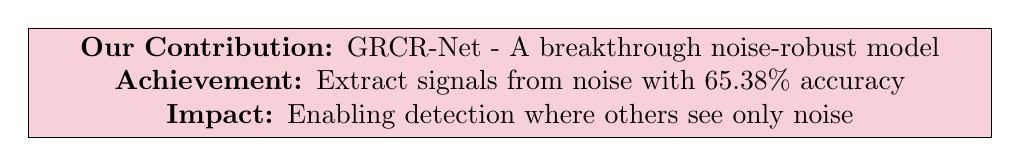
\begin{tikzpicture}[scale=0.8]
\node[draw,rectangle,fill=zjutred!20,text width=12cm,align=center] at (0,0) {
\textbf{Our Contribution:} GRCR-Net - A breakthrough noise-robust model \\
\textbf{Achievement:} Extract signals from noise with 65.38\% accuracy \\
\textbf{Impact:} Enabling detection where others see only noise
};
\end{tikzpicture}
\end{center}

\vspace{0.3cm}

\begin{center}
\textcolor{zjutred}{\large \textbf{Step 1 is the focus of this work - Building the noise-robust model!}}
\end{center}
\end{frame}



% Section 2: GRCR-Net Innovation Overview
\section{GRCR-Net Innovation Overview}


\begin{frame}{GRCR-Net: Three Core Innovations}
\begin{center}
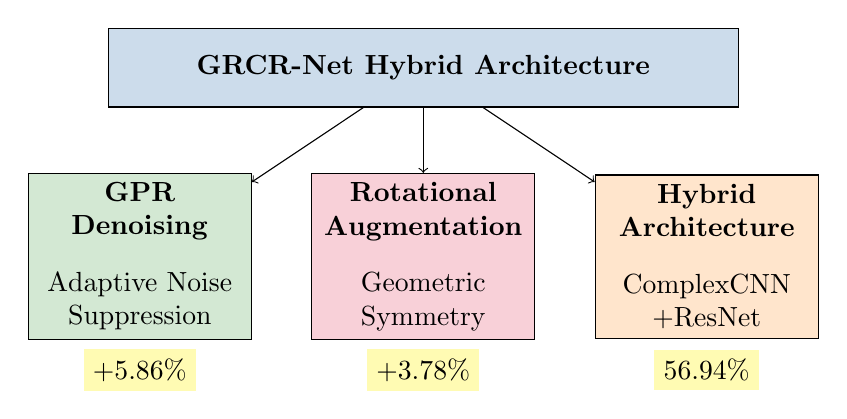
\begin{tikzpicture}[scale=1.2]
% Main framework
\node[draw,rectangle,fill=zjutblue!20,minimum width=8cm,minimum height=1cm] (main) at (0,0) {\textbf{GRCR-Net Hybrid Architecture}};

% Three innovation modules
\node[draw,rectangle,fill=zjutgreen!20,minimum width=2.8cm,minimum height=1.8cm] (gpr) at (-3,-2) {
\begin{minipage}{2.6cm}
\centering
\textbf{GPR Denoising}\\[0.3cm]
Adaptive Noise\\Suppression
\end{minipage}
};

\node[draw,rectangle,fill=zjutred!20,minimum width=2.8cm,minimum height=1.8cm] (aug) at (0,-2) {
\begin{minipage}{2.6cm}
\centering
\textbf{Rotational}\\
\textbf{Augmentation}\\[0.3cm]
Geometric Symmetry
\end{minipage}
};

\node[draw,rectangle,fill=orange!20,minimum width=2.8cm,minimum height=1.8cm] (hybrid) at (3,-2) {
\begin{minipage}{2.6cm}
\centering
\textbf{Hybrid}\\
\textbf{Architecture}\\[0.3cm]
ComplexCNN\\
+ResNet
\end{minipage}
};

% Connection lines
\draw[->] (main) -- (gpr);
\draw[->] (main) -- (aug);
\draw[->] (main) -- (hybrid);

% Performance improvement annotations
\node[fill=yellow!30] at (-3,-3.2) {+5.86\%};
\node[fill=yellow!30] at (0,-3.2) {+3.78\%};
% \node[fill=yellow!30] at (3,-3.2) {+8.27\%};
\node[fill=yellow!30] at (3,-3.2) {56.94\%};
\end{tikzpicture}
\end{center}

\vspace{0.5cm}
\begin{center}
\textcolor{zjutred}{\textbf{Final Performance: 65.38\% Accuracy,\\Surpassing State-of-the-Art}}
\end{center}
\end{frame}


% Section 3: Technical Details
\section{Core Technical Innovations}

\begin{frame}{GPR Denoising: Theoretical Foundation}
\begin{center}
\textcolor{zjutblue}{\Large \textbf{Part I: Signal Model and Assumptions}}
\end{center}

\vspace{0.5cm}
\textbf{Core Assumptions:}
\begin{enumerate}
\item \textbf{Additive White Gaussian Noise (AWGN):}
   \begin{equation}
   r[n] = s[n] + w[n]
   \end{equation}

\item \textbf{Independent Gaussian Distribution:} Each noise sample is independent and follows Gaussian distribution
   \begin{equation}
   w_I[n], w_Q[n] \sim \mathcal{N}(0, \sigma_n^2) \quad \text{(I/Q components)}
   \end{equation}

\item \textbf{Gaussian Process Modeling:} The entire signal can be modeled as a Gaussian Process
   \begin{equation}
   w[n] \sim \mathcal{CN}(0, \sigma_n^2) \quad \text{(Complex AWGN)}
   \end{equation}
\end{enumerate}

\vspace{0.3cm}
\begin{center}
\textcolor{zjutgreen}{\textbf{With these assumptions, we can derive the optimal noise estimation!}}
\end{center}
\end{frame}

\begin{frame}{GPR Denoising: Mathematical Derivation Process}
\begin{center}
\textcolor{zjutblue}{\Large \textbf{Part II: Complete Derivation Process}}
\end{center}

\vspace{0.1cm}
\begin{columns}
\begin{column}{0.45\textwidth}
\textbf{Step-by-Step Derivation:}

\vspace{0.1cm}
\textbf{1. I/Q Power Calculation:}
\begin{equation}
P_r = \frac{1}{M}\sum_{k=0}^{M-1}(r_I[k]^2 + r_Q[k]^2)
\end{equation}

\textbf{2. SNR Power Ratio:}
\begin{equation}
\text{SNR}_{\text{linear}} = 10^{\text{SNR}_{\text{dB}}/10}
\end{equation}

\textbf{3. Noise Power Calculation:}
\begin{equation}
P_w = \frac{P_r}{10^{\text{SNR}_{\text{dB}}/10} + 1}
\end{equation}

\textbf{4. Gaussian Noise Estimation:}
\begin{equation}
\sigma_n = \sqrt{\frac{P_w}{2}}
\end{equation}
\end{column}
% \begin{column}{0.55\textwidth}
% \vspace{-1cm}
\begin{column}{0.58\textwidth}
\vspace{-1.2cm}
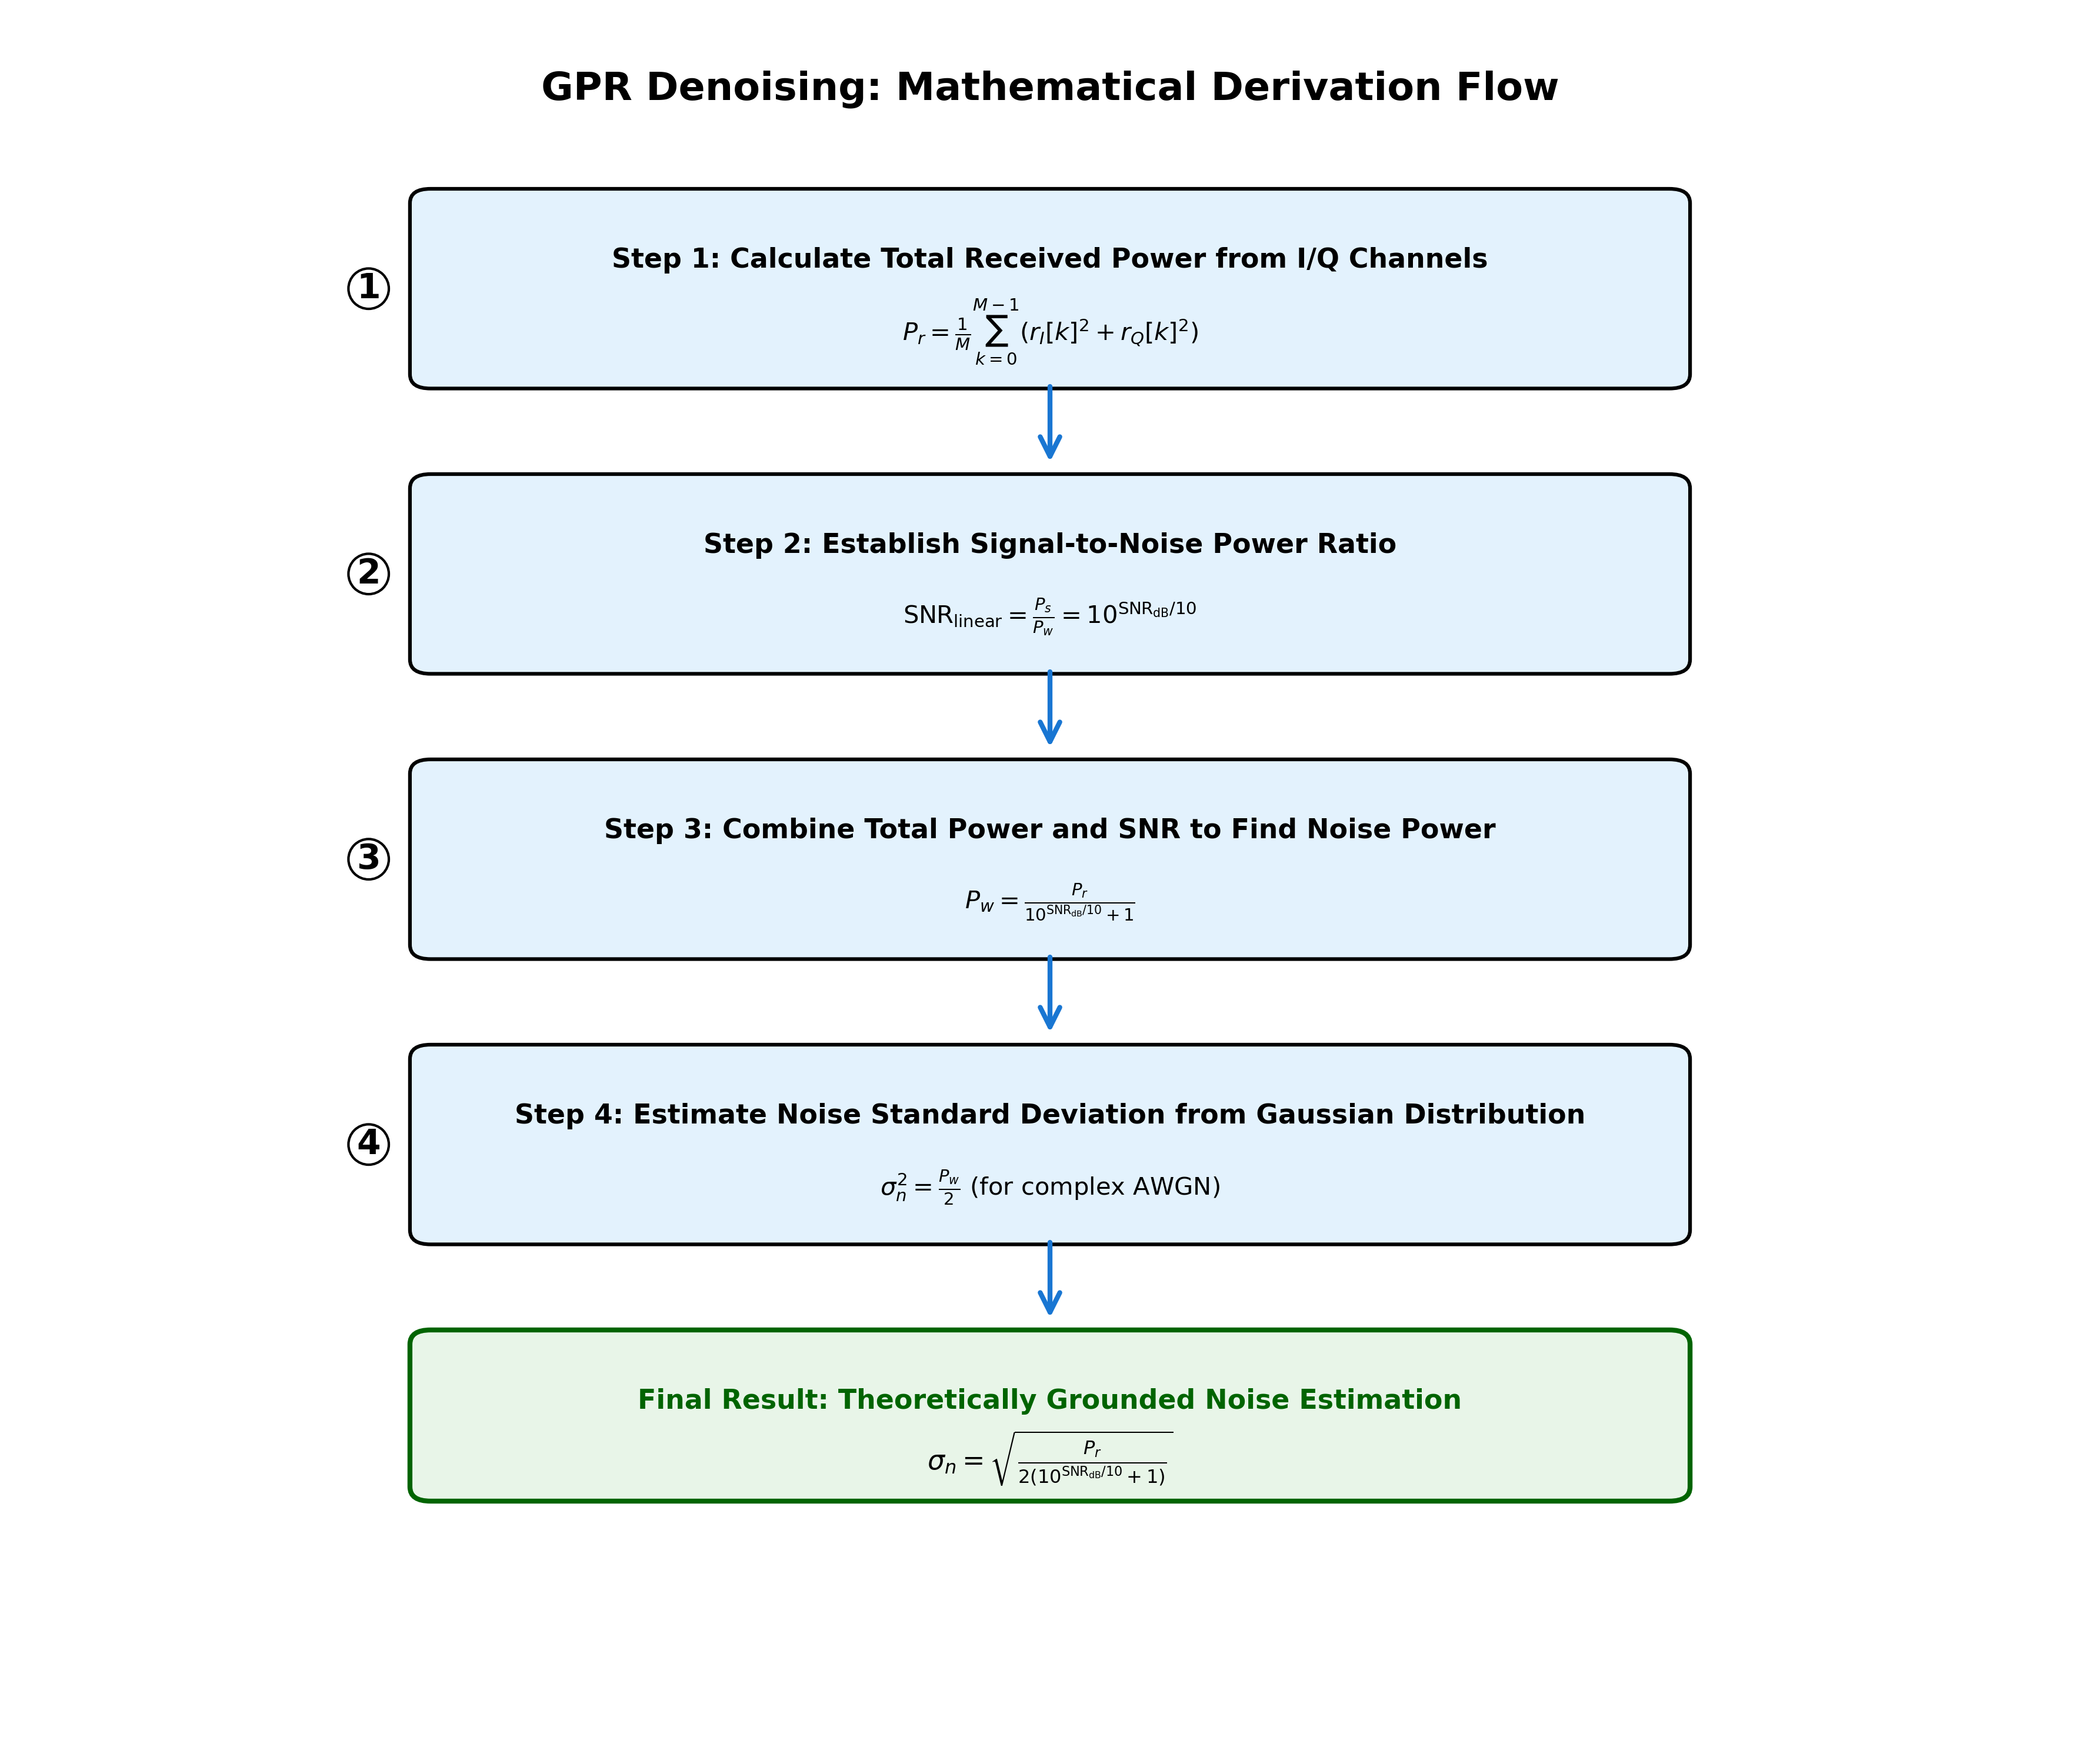
\includegraphics[width=\textwidth]{figure/gpr_derivation_flow.png}
\end{column}
\end{columns}
\end{frame}


\begin{frame}{GPR Denoising: Final Noise Estimation}
\textbf{Step 4: Estimate Noise Standard Deviation from Gaussian Distribution}

Since noise follows Gaussian distribution, for complex AWGN:
\begin{equation}
P_w = \mathbb{E}[|w[n]|^2] = \mathbb{E}[w_I^2[n]] + \mathbb{E}[w_Q^2[n]] = 2\sigma_n^2
\end{equation}

Therefore, the noise variance for each component:
\begin{equation}
\sigma_n^2 = \frac{P_w}{2} = \frac{P_r}{2(10^{\text{SNR}_{\text{dB}}/10} + 1)}
\end{equation}

\vspace{0.1cm}
\textbf{Final Noise Standard Deviation:}
\begin{equation}
\boxed{\sigma_n = \sqrt{\frac{P_r}{2(10^{\text{SNR}_{\text{dB}}/10} + 1)}}}
\end{equation}

% \vspace{0.05cm}
\begin{center}
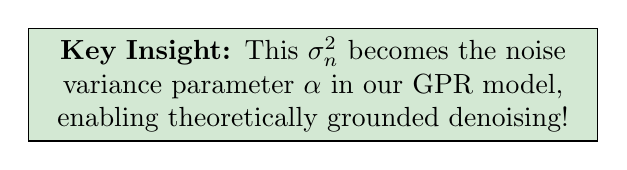
\begin{tikzpicture}[scale=0.7]
\node[draw,rectangle,fill=zjutgreen!20,text width=7cm,align=center] at (0,0) {
\textbf{Key Insight:} This $\sigma_n^2$ becomes the noise variance parameter $\alpha$ in our GPR model, enabling theoretically grounded denoising!
};
\end{tikzpicture}
\end{center}
\end{frame}

\begin{frame}{GPR Denoising: Adaptive Length Scale Strategy}
\textbf{RBF Kernel Function:}
\begin{equation}
k(x_i, x_j) = \sigma_f^2 \exp\left(-\frac{(x_i - x_j)^2}{2L^2}\right)
\end{equation}

% \vspace{0.2cm}
\textbf{Length Scale $L$ Controls Smoothing Strength:}
\begin{itemize}
\item Large $L$ $\rightarrow$ Strong smoothing, risk of oversmoothing
\item Small $L$ $\rightarrow$ Weak smoothing, preserves signal details
\end{itemize}

% \vspace{0.2cm}
\textbf{Problems with Fixed Large $L$ at Low SNR:}
\begin{enumerate}
\item \textcolor{zjutred}{Oversmoothing of signal features}
\item \textcolor{zjutred}{Loss of time-domain details}
\item \textcolor{zjutred}{Loss of critical phase information}
\end{enumerate}

% \vspace{0.2cm}
\textbf{Our Adaptive Strategy:}
\begin{equation}
L = \begin{cases}
L_0 & \text{if SNR} \geq 0 \text{ dB} \\
\max(L_{\min}, L_0(1 + \text{SNR}/20)) & \text{if SNR} < 0 \text{ dB}
\end{cases}
\end{equation}

\textcolor{zjutgreen}{\textbf{Key Insight:}} Lower SNR $\rightarrow$ Smaller $L$ $\rightarrow$ Preserve more signal details!
\end{frame}

\begin{frame}{Innovation 1: Complete GPR Denoising Pipeline}
\begin{columns}
\begin{column}{0.6\textwidth}
\textbf{Complete Algorithm:}
\begin{enumerate}
\item \textbf{Power Estimation}: $P_r = \frac{1}{M}\sum_{k=0}^{M-1}(r_I[k]^2+r_Q[k]^2)$
\item \textbf{Noise Variance}: $\sigma_n^2 = \frac{P_r}{2(10^{\text{SNR}/10} + 1)}$
\item \textbf{Adaptive Length Scale}: $L = \max(L_{\min}, L_0(1 + \text{SNR}/20))$
\item \textbf{GPR Denoising}: Apply to I and Q components separately
\item \textbf{Signal Reconstruction}: $\hat{s}[n] = \hat{s}_I[n] + j\hat{s}_Q[n]$
\end{enumerate}

\vspace{0.1cm}
\textbf{Key Advantages:}
\begin{itemize}
% \setlength{\itemsep}{0.1em}
\setlength{\itemsep}{0em}
\item \textcolor{zjutgreen}{Theoretically grounded noise estimation}
\item \textcolor{zjutgreen}{SNR-adaptive smoothing control}
\item \textcolor{zjutgreen}{Preserves signal feature integrity}
\item \textcolor{zjutgreen}{Optimal for different noise conditions}
\end{itemize}
\end{column}
\begin{column}{0.4\textwidth}
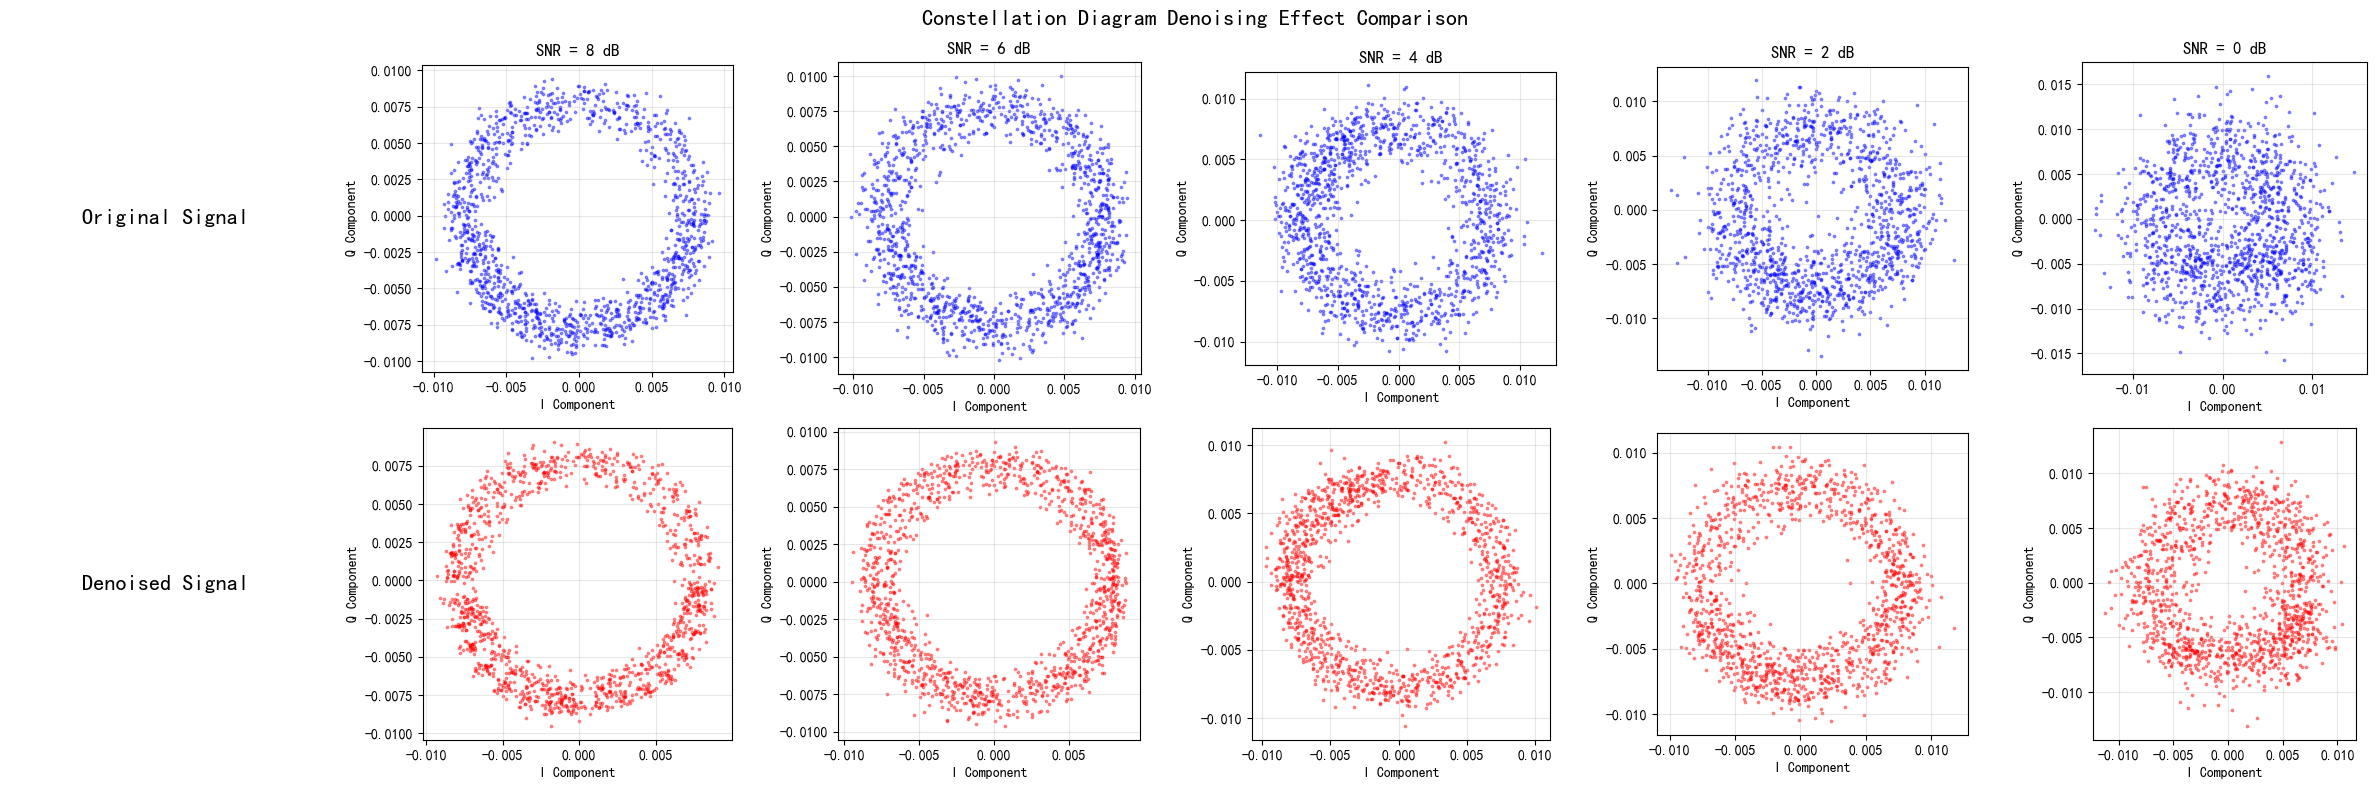
\includegraphics[width=\textwidth]{figure/constellation_denoising.png}

\vspace{0.3cm}
\begin{center}
\textcolor{zjutblue}{\textbf{Result: +5.86\% Accuracy Improvement}}
\end{center}
\end{column}
\end{columns}
\end{frame}

\begin{frame}{Innovation 2: Geometric Symmetry-Based Rotational Augmentation}
\begin{columns}
\begin{column}{0.5\textwidth}
\textbf{Theoretical Foundation:}
\begin{itemize}
\item Rotational symmetry of digital modulation constellations
\item Mathematical rigor of complex plane rotation
\item Exploitation of phase invariance
\end{itemize}

\textbf{Implementation:}
\begin{equation}
\begin{bmatrix} s'_I[n] \\ s'_Q[n] \end{bmatrix} = \begin{bmatrix} \cos\theta & -\sin\theta \\ \sin\theta & \cos\theta \end{bmatrix} \begin{bmatrix} s_I[n] \\ s_Q[n] \end{bmatrix}
\end{equation}

\textbf{Augmentation Strategy:}
\begin{itemize}
\item 90°, 180°, 270° rotations
\item 4× training data expansion
\item Applied to symmetric modulation types
\end{itemize}
\end{column}
\begin{column}{0.5\textwidth}
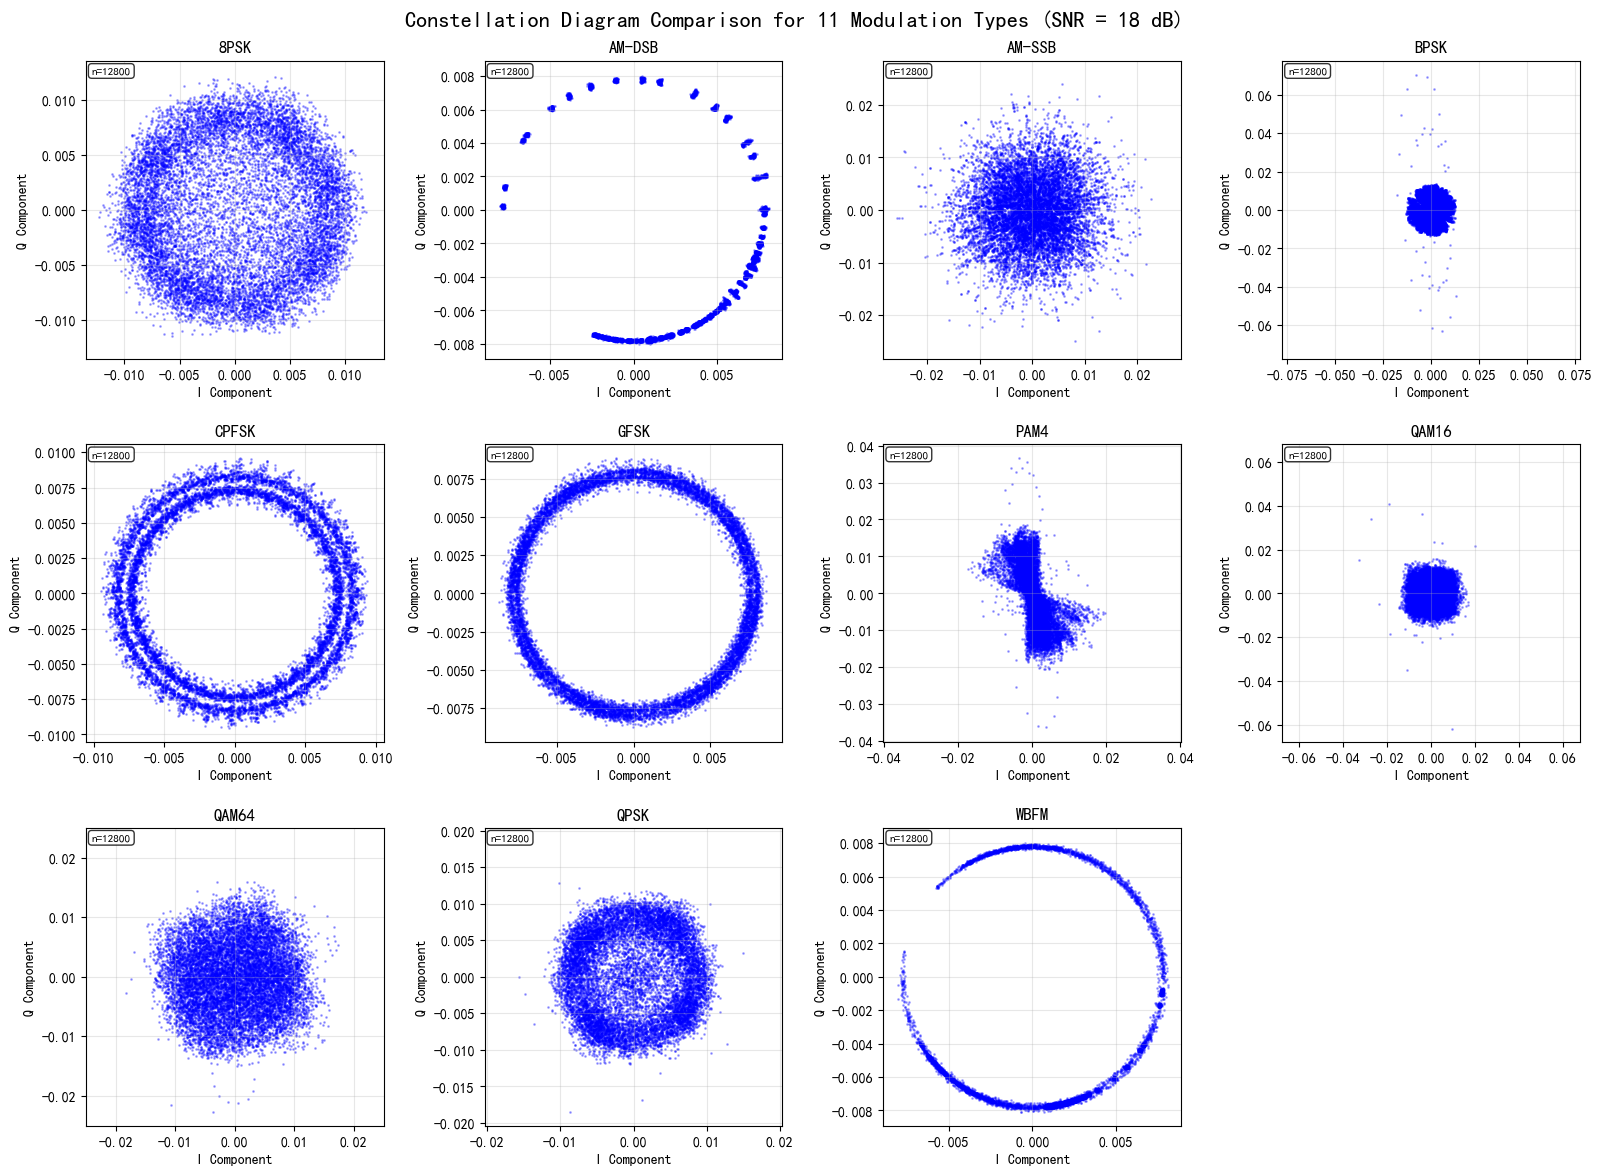
\includegraphics[width=\textwidth]{figure/constellation.png}
\end{column}
\end{columns}
\end{frame}

\begin{frame}{Innovation 3: Hybrid ComplexCNN-ResNet Architecture}
\begin{center}
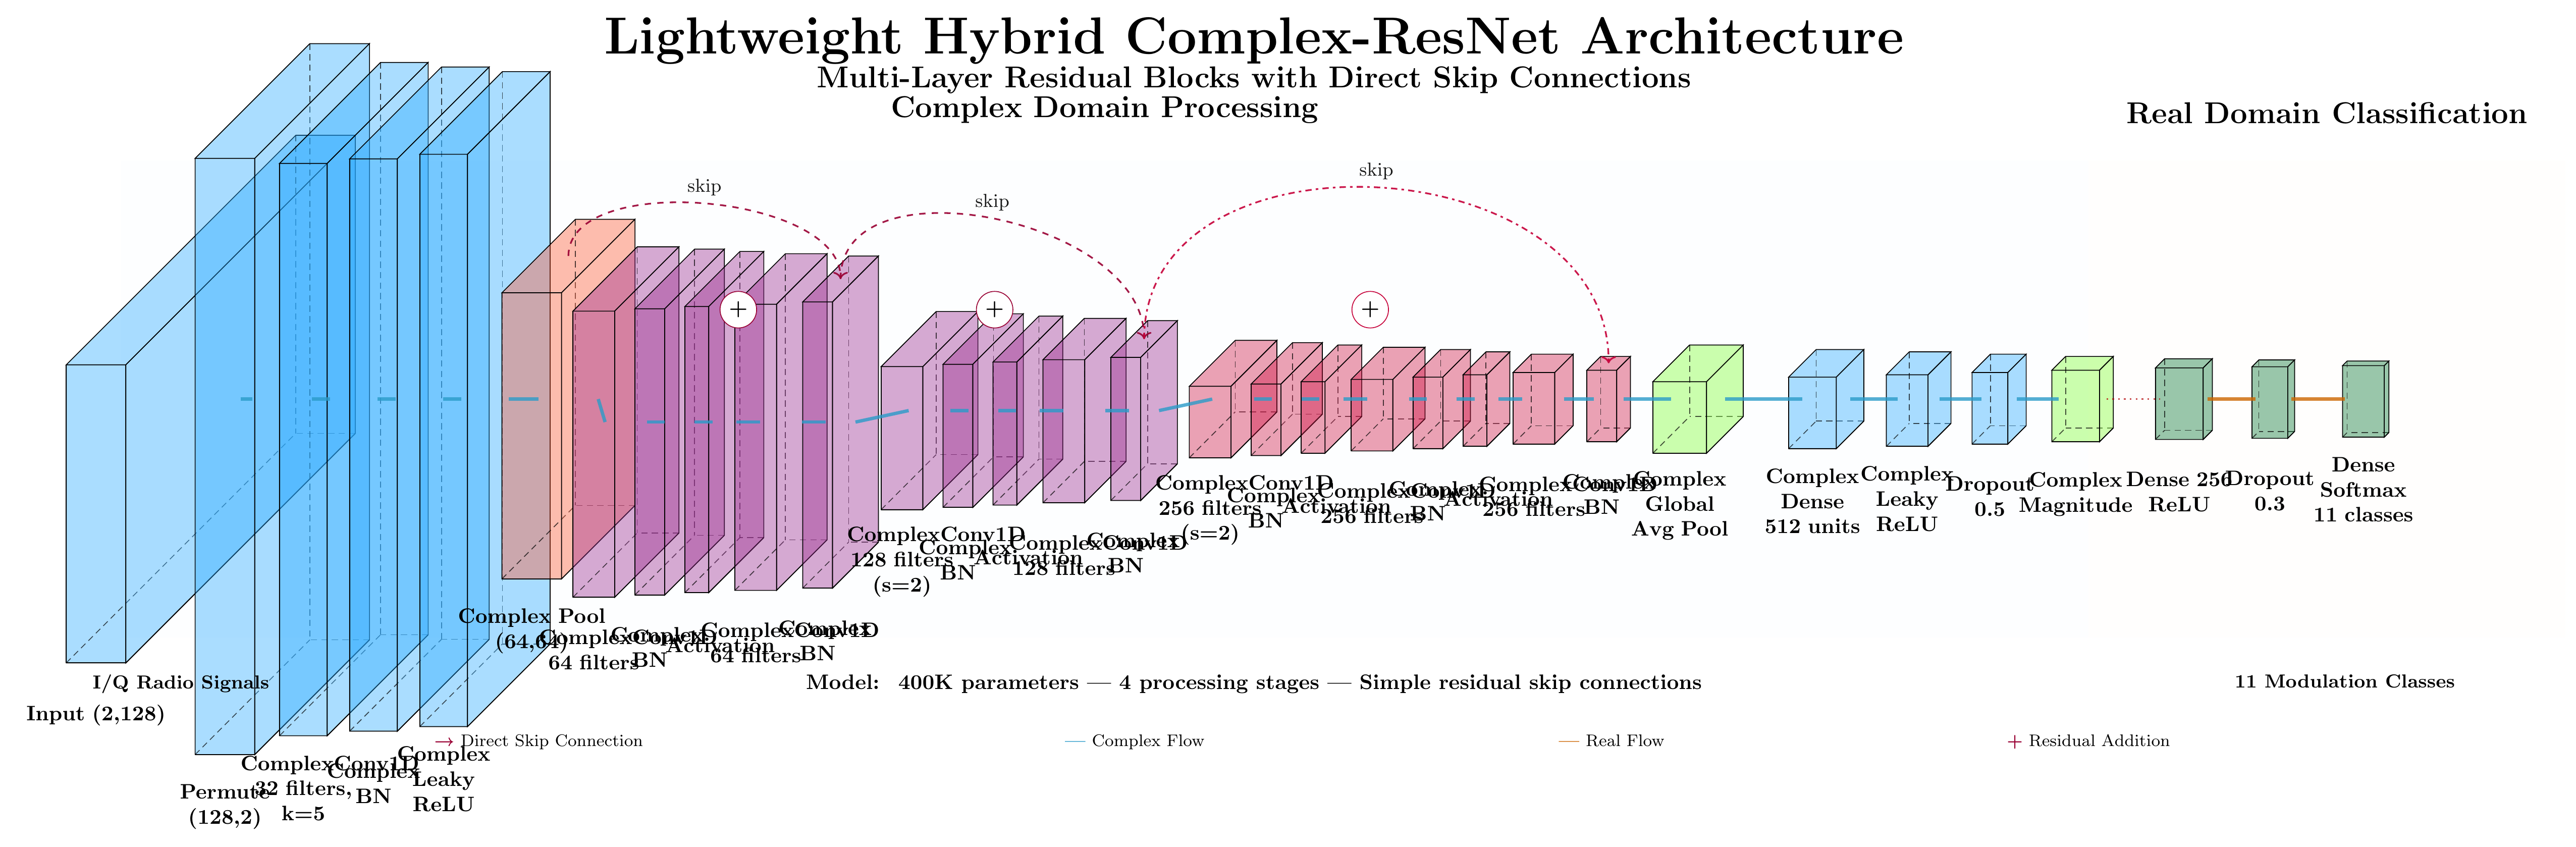
\includegraphics[width=0.8\textwidth]{figure/enhanced_hybrid_model.pdf}
\end{center}

\textbf{Design Principles:}
\begin{itemize}
\item \textbf{Complex Domain Processing}: Direct I/Q signal handling, preserving phase information
\item \textbf{Residual Learning}: Solving gradient vanishing in deep networks
\item \textbf{ModReLU Activation}: Maintaining complex geometric structure
\item \textbf{Lightweight Design}: Balancing performance and computational efficiency
\end{itemize}
\end{frame}

% Section 4: Experimental Results
\section{Experimental Results and Analysis}

\begin{frame}{Dataset and Experimental Setup}
\begin{columns}
\begin{column}{0.6\textwidth}
\textbf{RML2016.10a Dataset:}
\begin{itemize}
\item 11 modulation types
\item SNR range: -20dB to +18dB
\item 128 complex samples per signal
\item Data split: 72\%/8\%/20\%
\end{itemize}

\textbf{Experimental Environment:}
\begin{itemize}
\item Intel Core i9-13900K
\item NVIDIA GeForce RTX 4090 (24GB)
\item TensorFlow 2.17.0 + Keras 3.6.0
\item Ubuntu 24.04.2 LTS
\end{itemize}
\end{column}
\begin{column}{0.4\textwidth}
\begin{table}[h]
\centering
\scriptsize
\begin{tabular}{@{}cc@{}}
\toprule
Modulation & Samples \\
\midrule
8PSK & 22,000 \\
AM-DSB & 22,000 \\
AM-SSB & 22,000 \\
BPSK & 22,000 \\
CPFSK & 22,000 \\
GFSK & 22,000 \\
PAM4 & 22,000 \\
QAM16 & 22,000 \\
QAM64 & 22,000 \\
QPSK & 22,000 \\
WBFM & 22,000 \\
\bottomrule
\end{tabular}
\end{table}
\end{column}
\end{columns}
\end{frame}

\begin{frame}{Baseline Model Performance Comparison}
\begin{columns}
\begin{column}{0.5\textwidth}
\begin{table}[h]
\centering
\begin{tabular}{@{}cc@{}}
\toprule
\textbf{Model Architecture} & \textbf{Accuracy (\%)} \\
\midrule
FCNN & 42.65 \\
CNN2D & 47.31 \\
Transformer & 47.86 \\
CNN1D & 54.94 \\
ResNet & 55.37 \\
ComplexCNN & 57.11 \\
\midrule
\textcolor{zjutred}{\textbf{GRCR-Net}} & \textcolor{zjutred}{\textbf{65.38}} \\
\bottomrule
\end{tabular}
\end{table}
\end{column}
\begin{column}{0.5\textwidth}
\textbf{Key Findings:}
\begin{itemize}
\item ComplexCNN shows natural advantage for I/Q signals
\item ResNet's residual connections improve training stability
\item \textcolor{zjutred}{\textbf{GRCR-Net achieves 8.27\% improvement over best baseline}}
\end{itemize}

\vspace{0.5cm}
\textbf{Performance Breakthrough:}
\begin{itemize}
\item Surpasses existing SOTA methods
\item Consistent improvement across all SNR conditions
\item Exceptional performance in low SNR environments
\end{itemize}
\end{column}
\end{columns}
\end{frame}

\begin{frame}{Ablation Study: Component Contribution Analysis}
\begin{center}
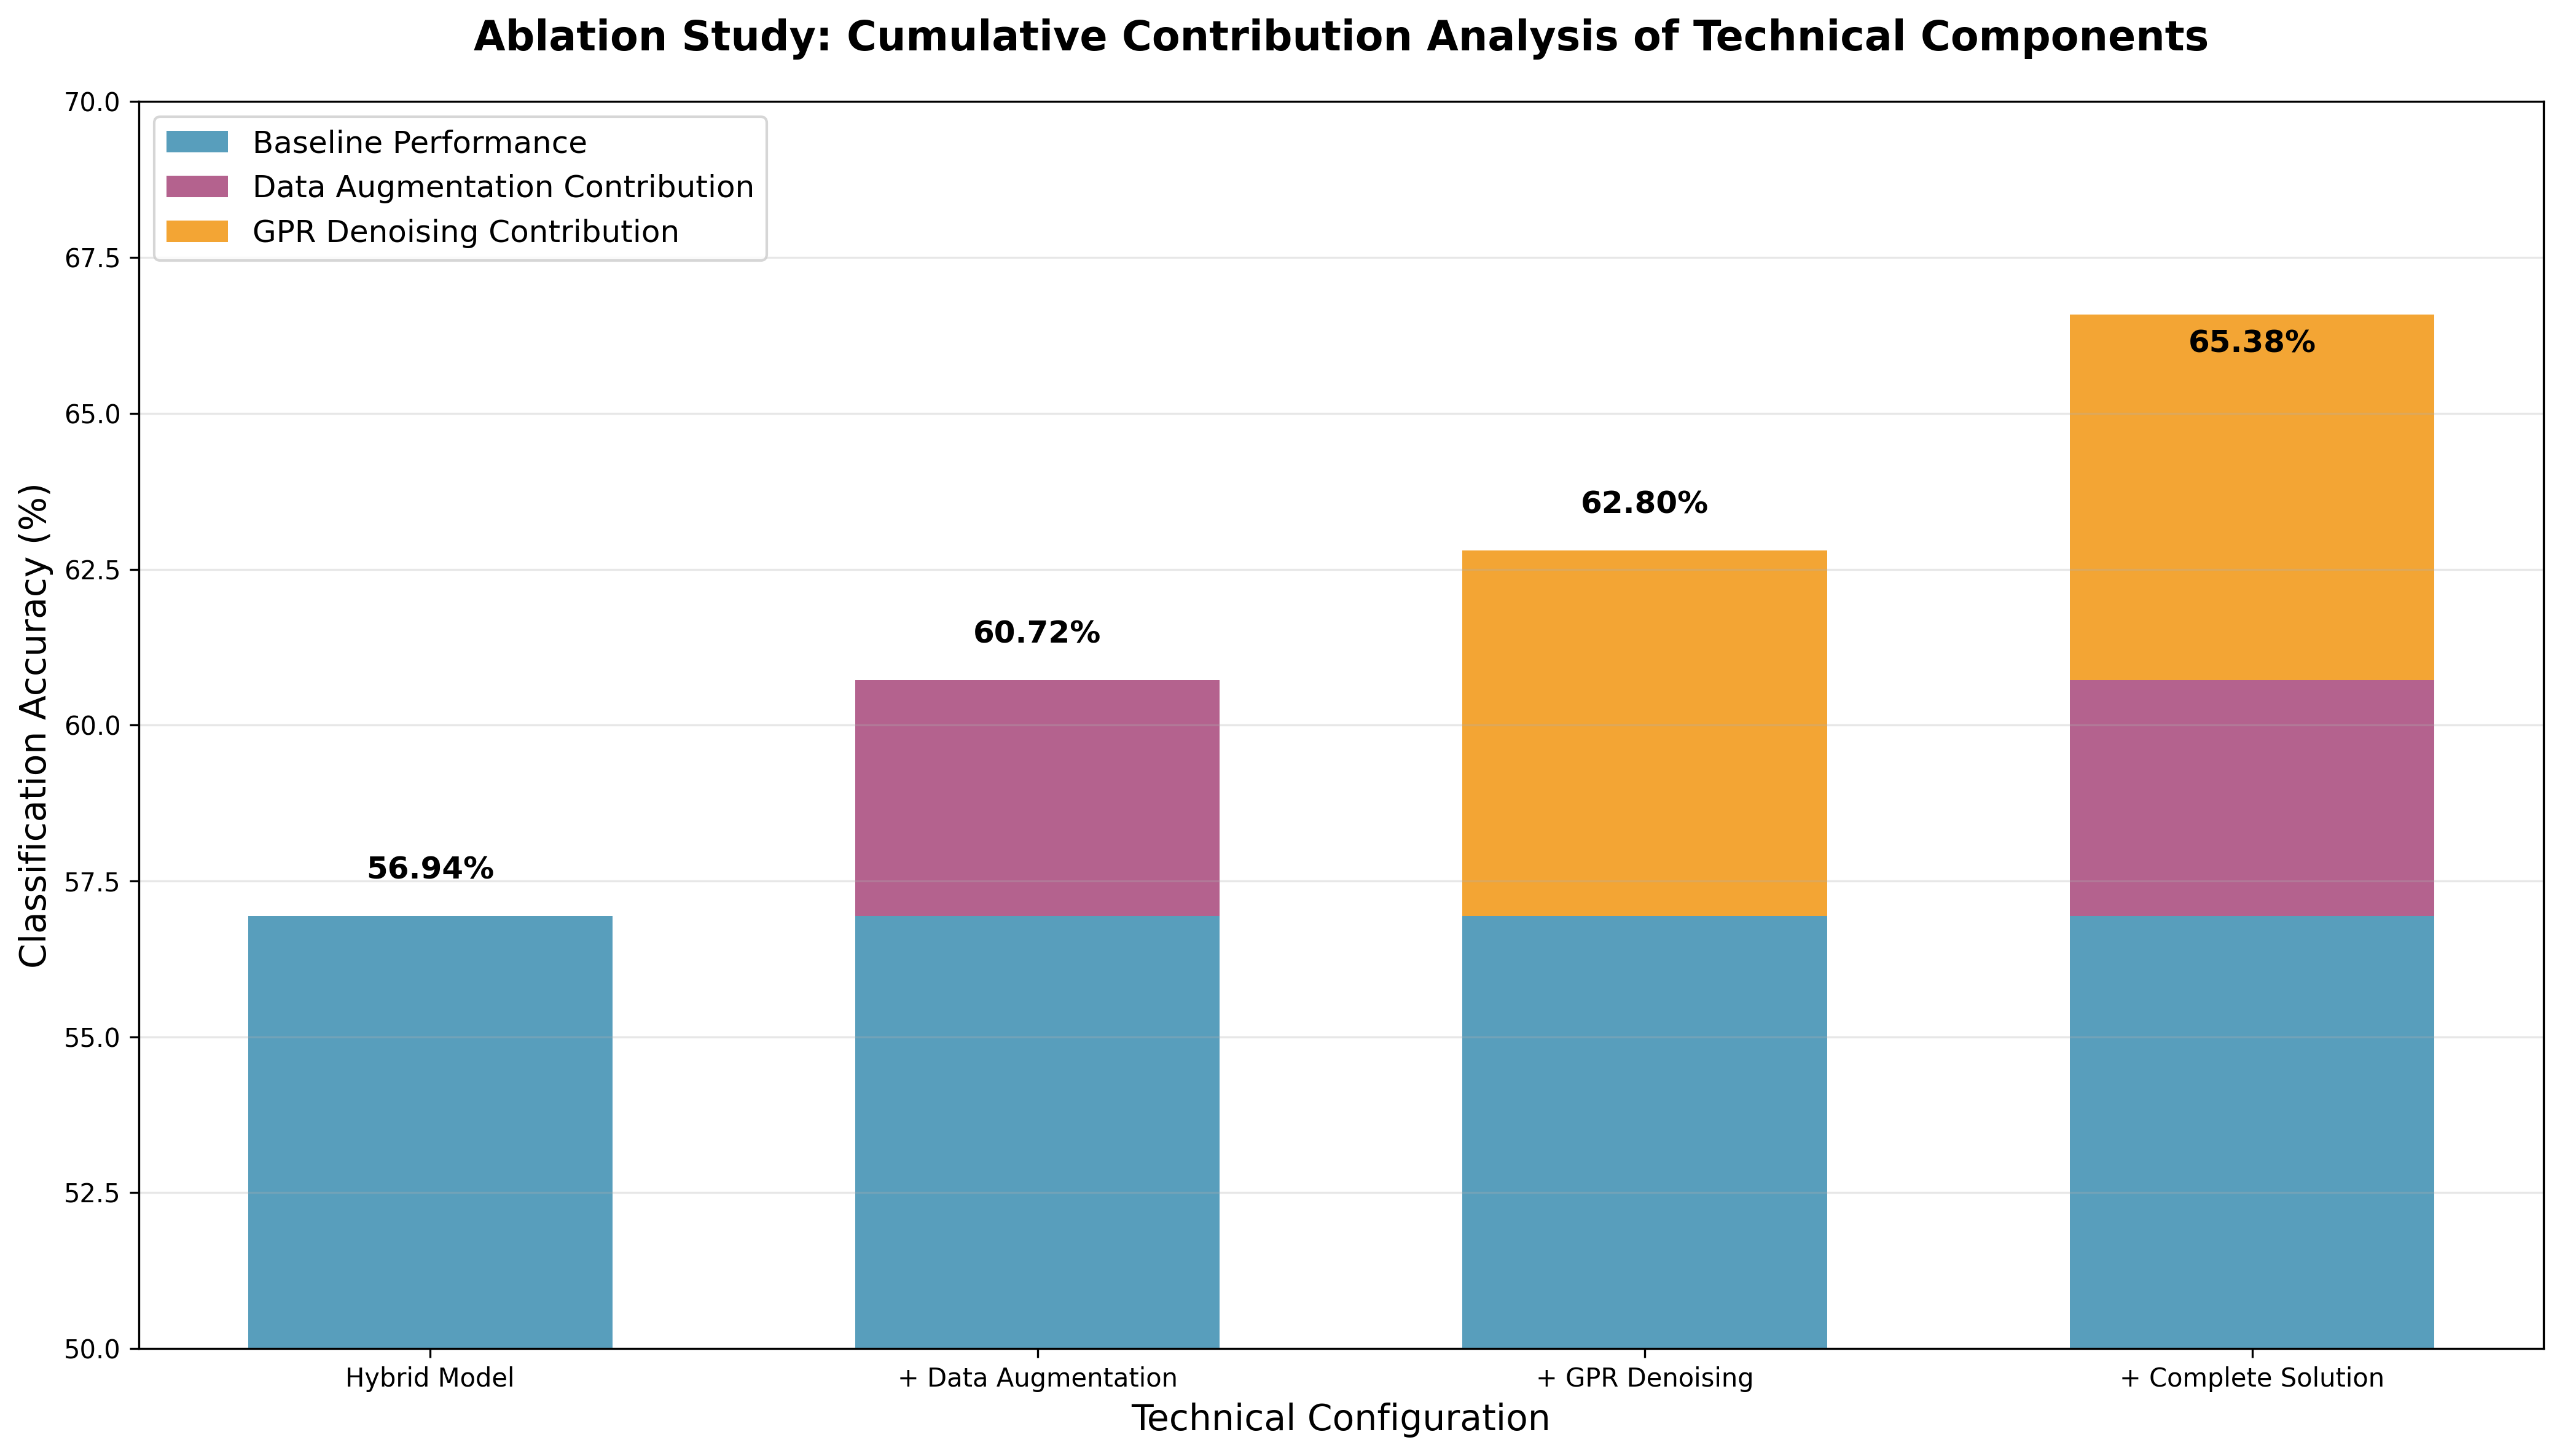
\includegraphics[width=0.6\textwidth]{figure/stacked_ablation_analysis.pdf}
\end{center}

\textbf{Key Insights:}
\begin{itemize}
\item GPR denoising contributes most: +5.86 percentage points
\item Rotational augmentation provides stable improvement: +3.78 percentage points
\item Synergistic effect of both techniques: total improvement of 8.44 percentage points
\end{itemize}
\end{frame}

\begin{frame}{Performance Across Different SNR Conditions}
\begin{center}
\textcolor{zjutblue}{\Large \textbf{GPR Denoising Performance Analysis}}
\end{center}

\vspace{0.5cm}
\begin{center}
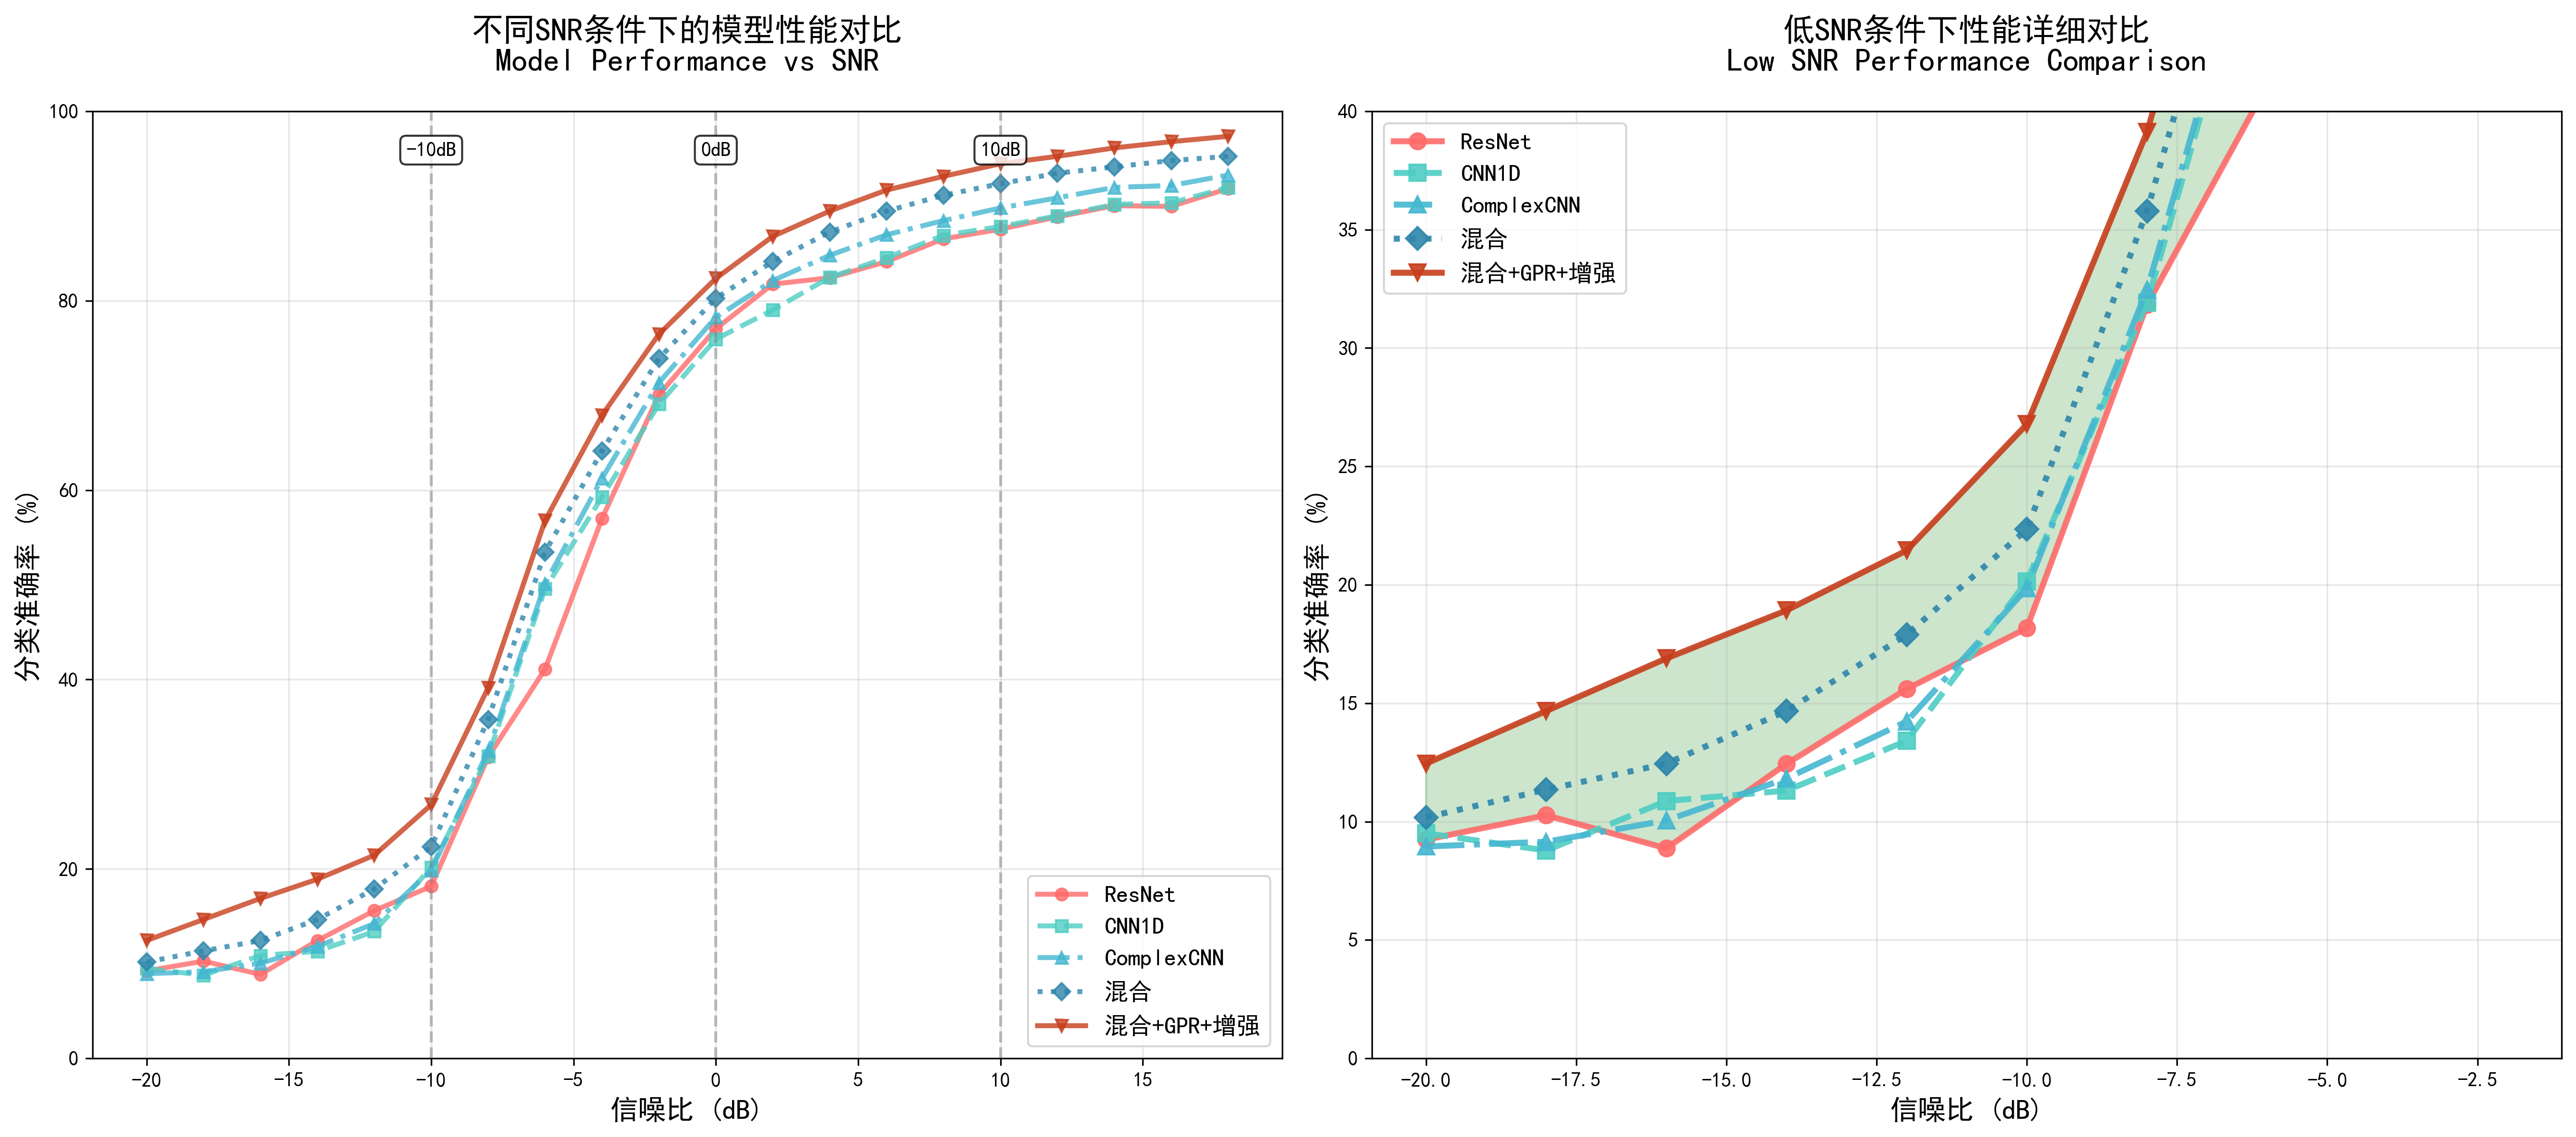
\includegraphics[width=0.85\textwidth]{figure/snr_performance_comparison.pdf}
\end{center}

\vspace{0.3cm}
\begin{center}
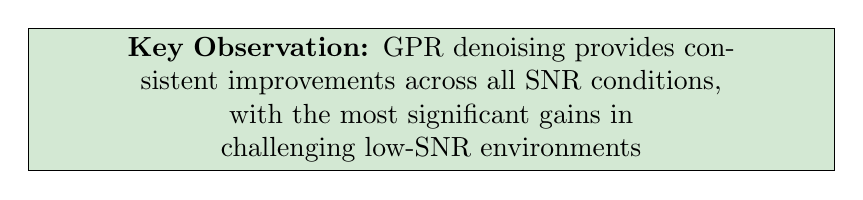
\begin{tikzpicture}[scale=0.8]
\node[draw,rectangle,fill=zjutgreen!20,text width=10cm,align=center] at (0,0) {
\textbf{Key Observation:} GPR denoising provides consistent improvements across all SNR conditions, \\
with the most significant gains in challenging low-SNR environments
};
\end{tikzpicture}
\end{center}
\end{frame}

\begin{frame}{Detailed SNR Performance Analysis}
\begin{columns}
\begin{column}{0.5\textwidth}
\centering
\tiny
\begin{tabular}{@{}cccc@{}}
\toprule
\textbf{SNR} & \textbf{Base} & \textbf{+GPR} & \textbf{Gain} \\
\midrule
-20 & 8.93 & 9.96 & +1.03 \\
-18 & 8.68 & 10.22 & +1.54 \\
-16 & 9.85 & 12.69 & +2.84 \\
-14 & 11.08 & 17.32 & +6.24 \\
-12 & 12.65 & 24.18 & +11.53 \\
-10 & 20.15 & 35.05 & +14.90 \\
-8 & 34.66 & 47.36 & +12.70 \\
-6 & 54.86 & 61.21 & +6.35 \\
-4 & 64.02 & 70.84 & +6.82 \\
-2 & 75.66 & 80.89 & +5.23 \\
0 & 79.43 & 83.17 & +3.74 \\
2 & 82.96 & 87.07 & +4.11 \\
4 & 84.56 & 89.00 & +4.44 \\
6 & 83.93 & 89.38 & +5.45 \\
8 & 83.17 & 89.10 & +5.93 \\
10 & 84.73 & 89.85 & +5.12 \\
12 & 85.81 & 90.31 & +4.50 \\
14 & 85.31 & 88.81 & +3.50 \\
16 & 82.25 & 88.15 & +5.90 \\
18 & 83.87 & 88.98 & +5.11 \\
\bottomrule
\end{tabular}
\end{column}
\begin{column}{0.5\textwidth}
\textbf{Key Findings:}

\vspace{0.2cm}

\textbf{\textcolor{zjutred}{Low SNR (-20 to -8dB):}}
\begin{itemize}
\footnotesize
\setlength{\itemsep}{0pt}
\item Peak: \textbf{+14.90\%} at -10dB
\item Average: \textbf{7.25\%}
\end{itemize}

\textbf{\textcolor{zjutblue}{Medium SNR (-6 to 4dB):}}
\begin{itemize}
\footnotesize
\setlength{\itemsep}{0pt}
\item Range: 3.74\% to 6.82\%
\item Average: \textbf{5.12\%}
\end{itemize}

\textbf{\textcolor{zjutgreen}{High SNR (6 to 18dB):}}
\begin{itemize}
\footnotesize
\setlength{\itemsep}{0pt}
\item Range: 3.50\% to 5.93\%
\item Average: \textbf{5.07\%}
\end{itemize}

\vspace{0.2cm}

% \begin{center}
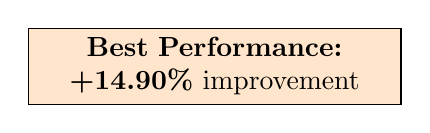
\begin{tikzpicture}[scale=0.7]
\node[draw,rectangle,fill=orange!20,text width=4.5cm,align=center] at (0,0) {
\textbf{Best Performance:} \\
\textbf{+14.90\%} improvement
};
\end{tikzpicture}
% \end{center}
\end{column}
\end{columns}
\end{frame}

\begin{frame}{Training Convergence Analysis}
\begin{columns}
\begin{column}{0.55\textwidth}
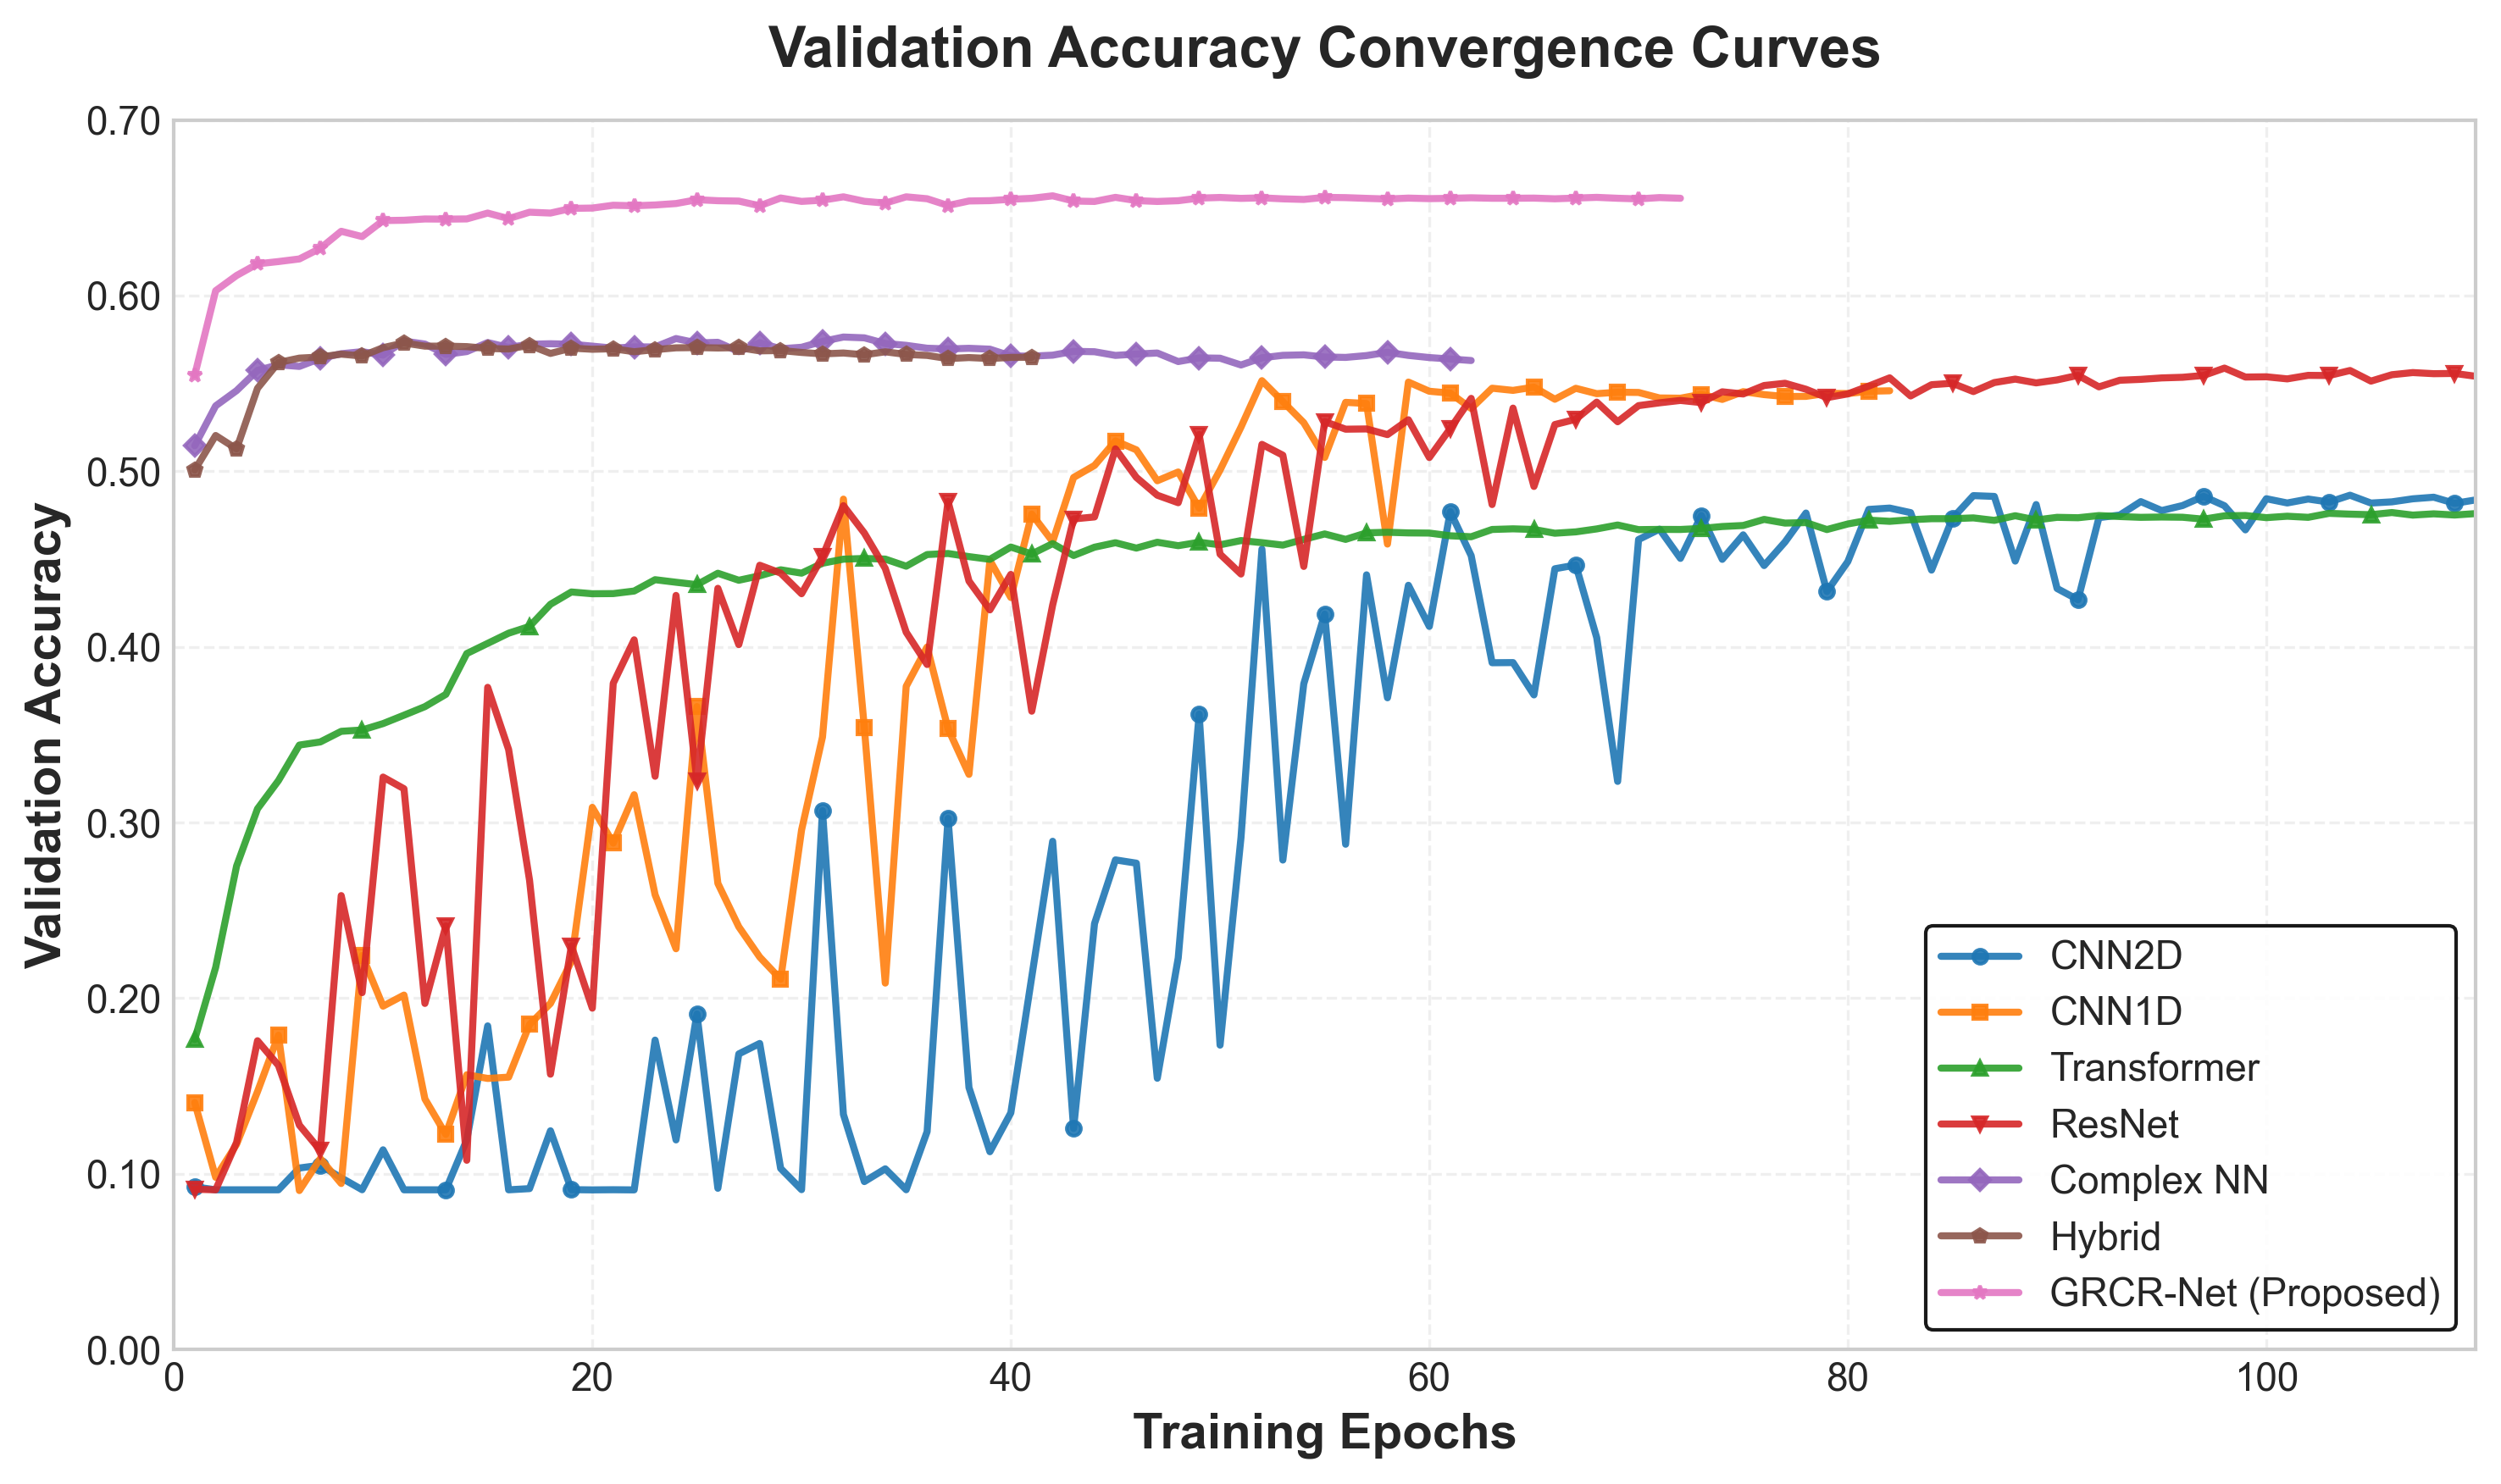
\includegraphics[width=\textwidth]{figure/validation_accuracy_convergence.pdf}
\end{column}
\begin{column}{0.45\textwidth}
\textbf{Key Insights:}
\begin{itemize}
\item \textcolor{zjutgreen}{\textbf{Fast Convergence}}: Optimal in 5-10 epochs
\item \textcolor{zjutgreen}{\textbf{Stable Training}}: Smooth without oscillations
\item \textcolor{zjutgreen}{\textbf{Best Performance}}: Outperforms all baselines
\item \textcolor{zjutgreen}{\textbf{Robust Results}}: Consistent across runs
\end{itemize}

\vspace{0.3cm}
\begin{center}
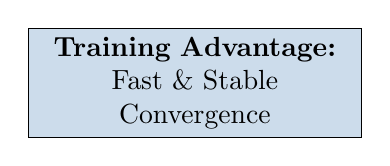
\begin{tikzpicture}[scale=0.7]
\node[draw,rectangle,fill=zjutblue!20,text width=4cm,align=center] at (0,0) {
\textbf{Training Advantage:} \\
Fast \& Stable Convergence
};
\end{tikzpicture}
\end{center}
\end{column}
\end{columns}
\end{frame}

% Section 5: Technical Contributions and Impact
\section{Technical Contributions and Impact}

\begin{frame}{Major Technical Contributions}
\begin{enumerate}
\item \textbf{Adaptive Noise Suppression Technology}
\begin{itemize}
\item First SNR-adaptive GPR denoising algorithm
\item Optimal denoising under different noise conditions
\item Novel approach for complex electromagnetic environments
\end{itemize}

\item \textbf{Geometric Property Data Augmentation Strategy}
\begin{itemize}
\item Exploits inherent symmetry of modulation signals
\item Significantly improves robustness to phase offset
\item Effective solution for data-scarce scenarios
\end{itemize}

\item \textbf{Hybrid Neural Network Architecture Innovation}
\begin{itemize}
\item First fusion of ComplexCNN and ResNet advantages
\item Deep residual learning in complex domain
\item New architectural paradigm for I/Q signal processing
\end{itemize}
\end{enumerate}
\end{frame}

\begin{frame}{Comparison with State-of-the-Art Methods}
\begin{table}[h]
\centering
\tiny
\begin{tabular}{@{}cccccc@{}}
\toprule
\textbf{Method} & \textbf{Accuracy(\%)} & \textbf{Year} & \textbf{Publication} & \textbf{Model Size} & \textbf{Key Technology} \\
\midrule
LDCVNN & 62.41 & 2025 & JCR Q2 & Lightweight & Dual-branch complex network \\
ULCNN & 62.47 & 2022 & JCR Q2 & Lightweight & Ultra-lightweight CNN \\
AMC-NET & 62.51 & 2023 & ICASSP (CCF B) & Normal & Frequency-domain denoising \\
HFECNET-CA & 63.92 & 2023 & JCR Q2 & Lightweight & Attention mechanism \\
AbFTNet (Previous SOTA) & 64.59 & 2024 & JCR Q2 & Normal & Multimodal fusion \\
\midrule
\textcolor{zjutred}{\textbf{GRCR-Net (Ours)}} & \textcolor{zjutred}{\textbf{65.38}} & \textcolor{zjutred}{\textbf{2025}} & \textcolor{zjutred}{\textbf{This Work}} & \textcolor{zjutred}{\textbf{Lightweight}} & \textcolor{zjutred}{\textbf{GPR+Rotation+Hybrid}} \\
\bottomrule
\end{tabular}
\end{table}

\vspace{0.5cm}
\textbf{Core Advantages:}
\begin{itemize}
\item \textcolor{zjutgreen}{\textbf{Performance Leadership}}: Surpasses best existing method by 0.79\%
\item \textcolor{zjutgreen}{\textbf{Technical Innovation}}: Organic fusion of three core technologies
\item \textcolor{zjutgreen}{\textbf{Practical Robustness}}: Stable performance in complex environments
\item \textcolor{zjutgreen}{\textbf{Scalability}}: Components can be applied independently
\end{itemize}
\end{frame}

\begin{frame}{Comprehensive Performance Comparison}
\begin{columns}
\begin{column}{0.6\textwidth}
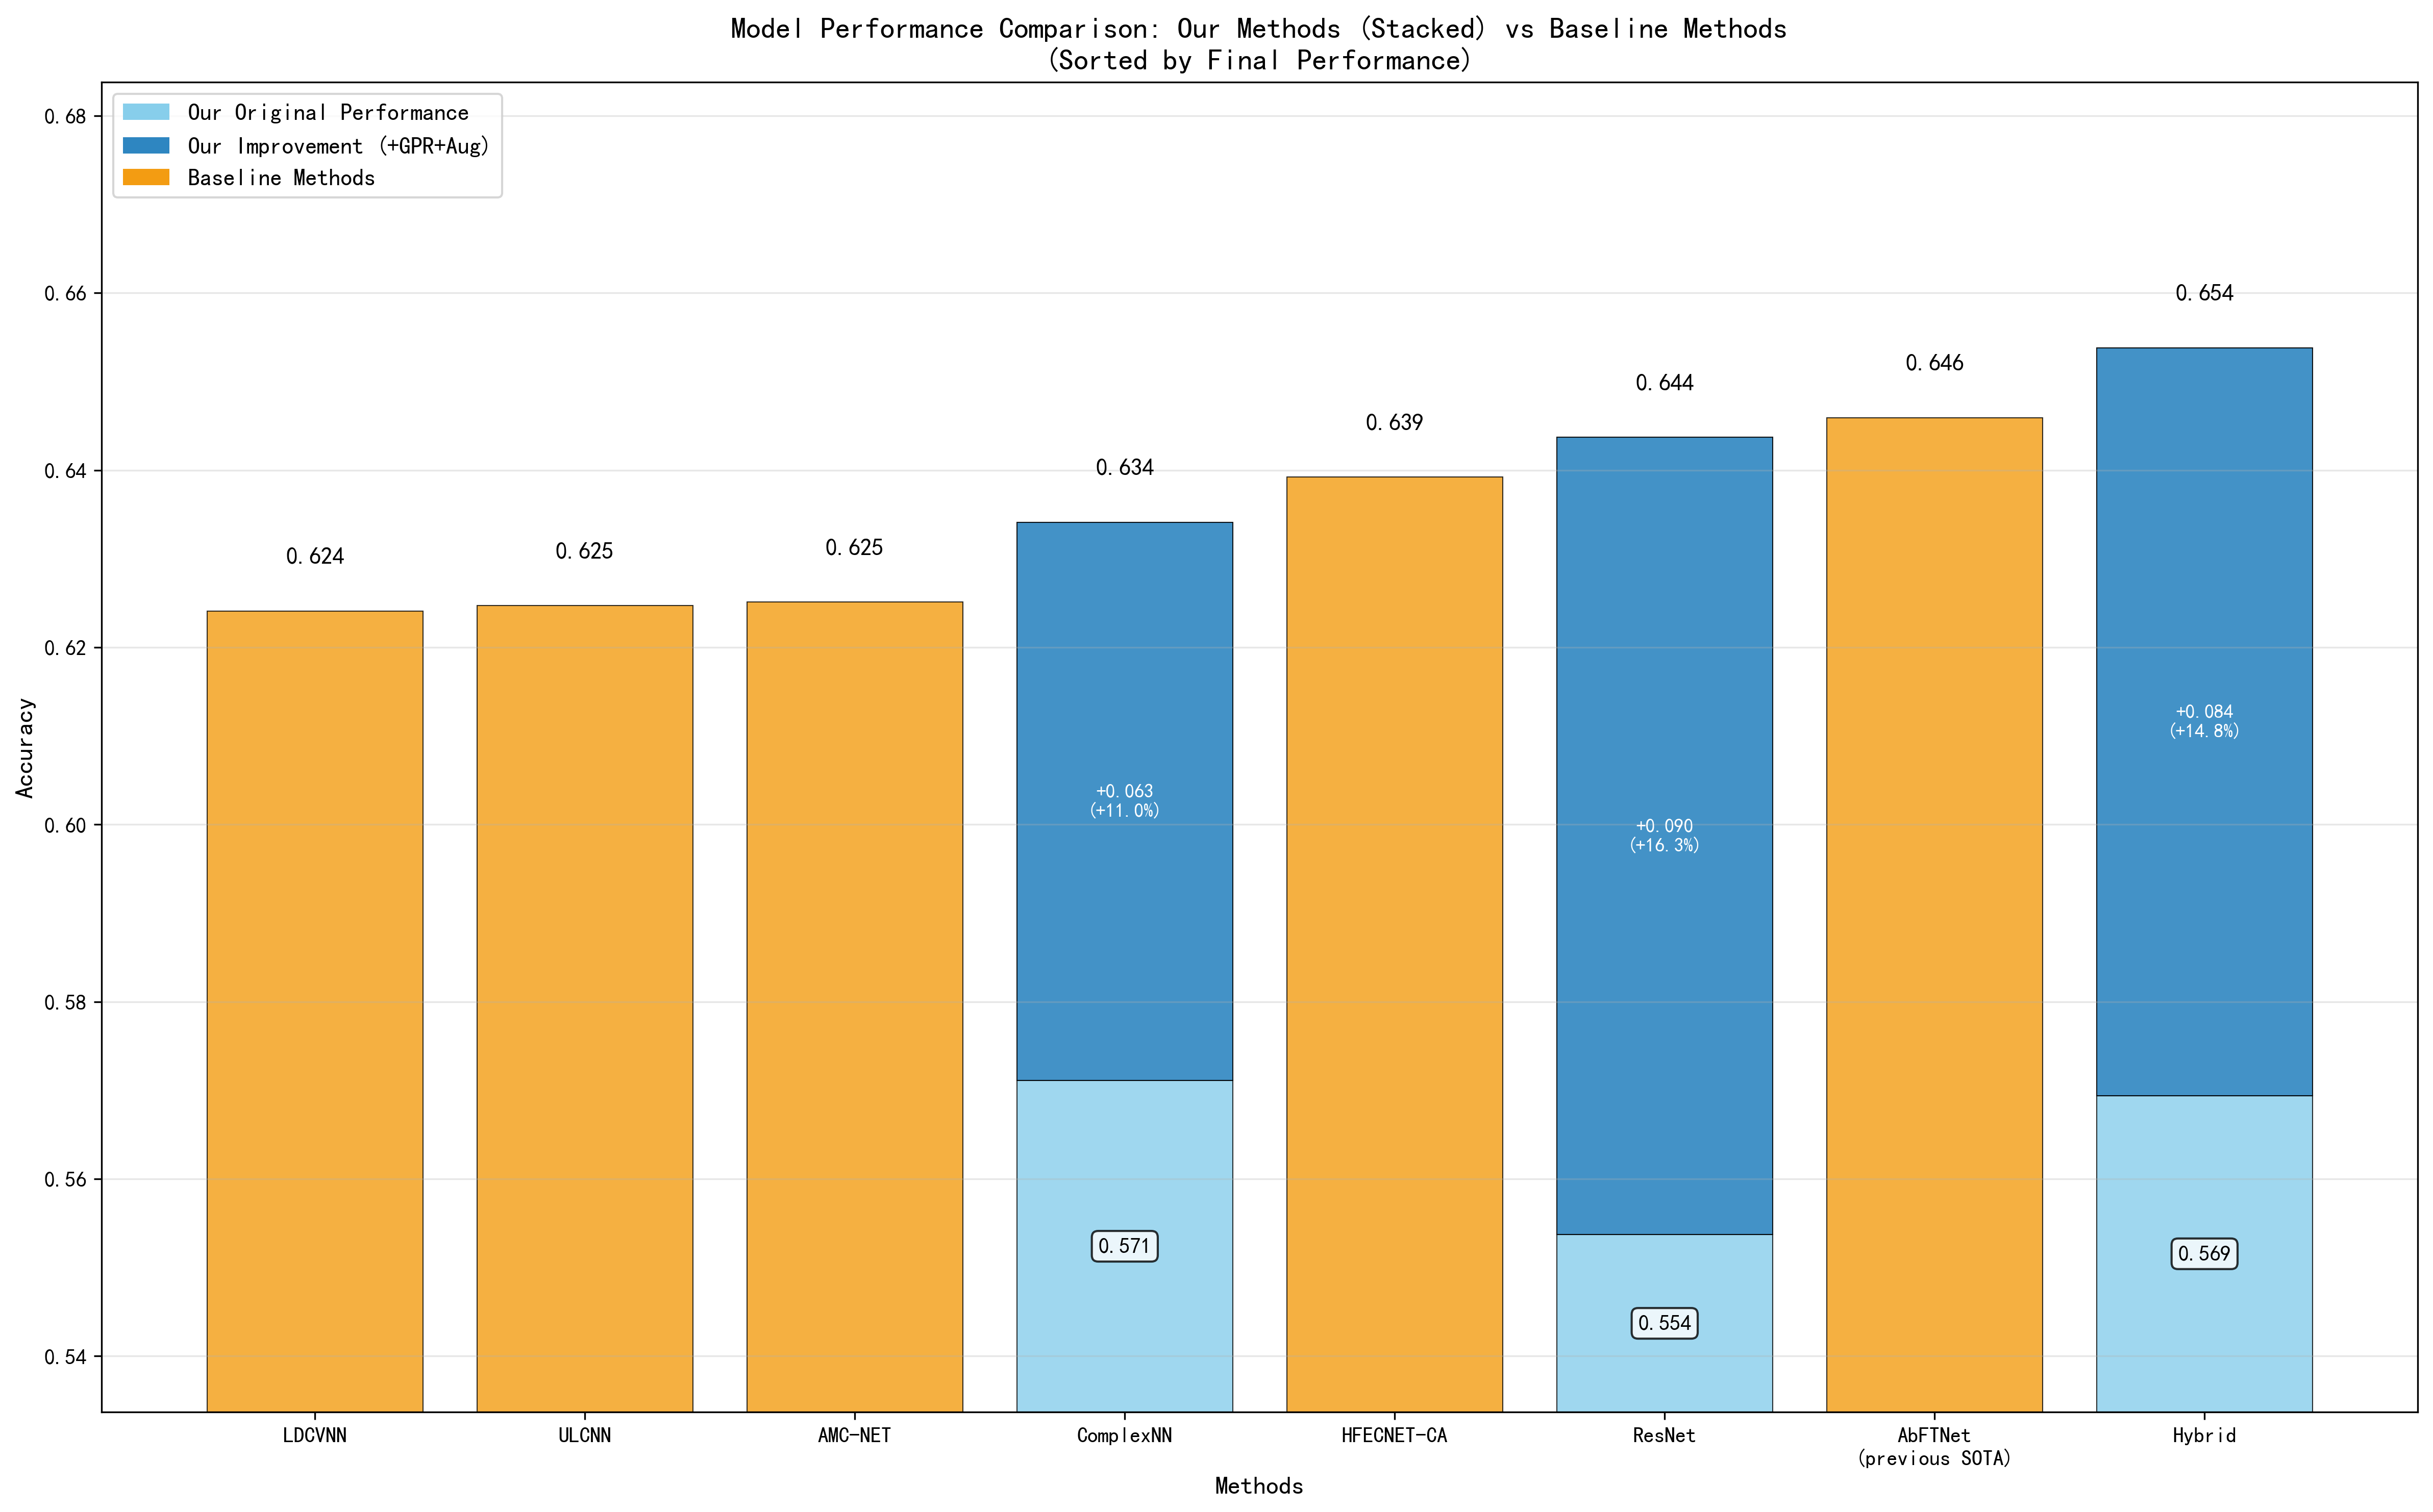
\includegraphics[width=\textwidth]{figure/sorted_stacked_comparison.png}
\end{column}
\begin{column}{0.4\textwidth}
\textbf{SOTA Achievement:}
\begin{itemize}
\item \textcolor{zjutred}{\textbf{65.38\%}} accuracy
\item \textcolor{zjutgreen}{\textbf{+0.79\%}} vs. AbFTNet (2024)
% \item \textcolor{zjutgreen}{\textbf{+1.46\%}} vs. HFECNET-CA (2023)
\item \textcolor{zjutgreen}{\textbf{+2.87\%}} vs. AMC-NET (2023)
\item \textcolor{zjutgreen}{\textbf{+2.91\%}} vs. ULCNN (2022)
\end{itemize}

\vspace{0.1cm}
\textbf{Key Advantages:}
\begin{itemize}
\item Clear performance leadership
\item Consistent improvements
\item Robust across conditions
\item New benchmark established
\end{itemize}

\vspace{0.1cm}
\begin{center}
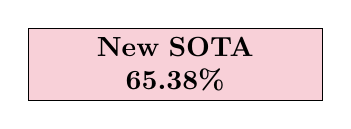
\begin{tikzpicture}[scale=0.6]
\node[draw,rectangle,fill=zjutred!20,text width=3.5cm,align=center] at (0,0) {
\textbf{New SOTA} \\
\textbf{65.38\%}
};
\end{tikzpicture}
\end{center}
\end{column}
\end{columns}
\end{frame}

% \begin{frame}{Practical Application Value and Prospects}
% \begin{columns}
% \begin{column}{0.6\textwidth}
% \textbf{Direct Application Domains:}
% \begin{itemize}
% \item \textbf{Cognitive Radio}: Intelligent spectrum sensing and management
% \item \textbf{Electronic Warfare}: Signal reconnaissance and identification
% \item \textbf{Communication Regulation}: Spectrum monitoring and compliance
% \item \textbf{5G/6G Networks}: Intelligent signal processing
% \end{itemize}

% \textbf{Technology Extension Value:}
% \begin{itemize}
% \item GPR denoising applicable to other signal processing tasks
% \item Hybrid architecture extendable to other complex signal analysis
% \item Rotational augmentation suitable for geometrically symmetric data
% \end{itemize}
% \end{column}
% \begin{column}{0.4\textwidth}
% \begin{tikzpicture}[scale=0.8]
% % Application scenario diagram
% \node[draw,circle,fill=zjutblue!20] (core) at (0,0) {GRCR-Net};
% \node[draw,rectangle,fill=zjutgreen!20,text width=2.0cm,align=center] (cr) at (-2,2) {Cognitive\\Radio};
% \node[draw,rectangle,fill=zjutgreen!20,text width=2.0cm,align=center] (ew) at (2,2) {Electronic\\Warfare};
% \node[draw,rectangle,fill=zjutgreen!20,text width=2.0cm,align=center] (sm) at (-2,-2) {Spectrum\\Regulation};
% \node[draw,rectangle,fill=zjutgreen!20,text width=2.0cm,align=center] (ng) at (2,-2) {Next-Gen\\Comm};

% \draw[->] (core) -- (cr);
% \draw[->] (core) -- (ew);
% \draw[->] (core) -- (sm);
% \draw[->] (core) -- (ng);
% \end{tikzpicture}
% \end{column}
% \end{columns}
% \end{frame}

% Section 6: Conclusion and Future Work
\section{Conclusion and Future Work}

\begin{frame}{Research Summary}
\begin{center}
\textcolor{zjutblue}{\Large \textbf{GRCR-Net: A Breakthrough AMC Method}}
\end{center}

\vspace{0.5cm}
\begin{columns}
\begin{column}{0.5\textwidth}
\textbf{Core Achievements:}
\begin{itemize}
\item[$\checkmark$] Achieved 65.38\% classification accuracy
\item[$\checkmark$] Surpassed existing SOTA methods
\item[$\checkmark$] Exceptional performance in low SNR environments
\item[$\checkmark$] Proposed three core technical innovations
\end{itemize}

\textbf{Technical Breakthroughs:}
\begin{itemize}
\item[$\bullet$] Adaptive GPR denoising algorithm
\item[$\bullet$] Geometric symmetry data augmentation
\item[$\bullet$] Hybrid ComplexCNN-ResNet architecture
\end{itemize}
\end{column}
\begin{column}{0.5\textwidth}
\textbf{Impact Significance:}
\begin{itemize}
\item[$\bullet$] Solution for complex electromagnetic environments
\item[$\bullet$] Advancement of cognitive radio technology
\item[$\bullet$] New insights for signal processing field
\item[$\bullet$] Important theoretical and practical value
\end{itemize}

\textbf{Open Source Contribution:}
\begin{itemize}
\item[$\bullet$] Complete code open-sourced
\item[$\bullet$] Detailed experimental data
\item[$\bullet$] Comprehensive technical documentation
\end{itemize}
\end{column}
\end{columns}
\end{frame}

\begin{frame}{Future Research Directions}
\begin{enumerate}
\item \textbf{Algorithm Optimization and Extension}
\begin{itemize}
\item Explore performance in more complex channel environments
\item Research real-time processing optimization strategies
\item Extend to more modulation types
\end{itemize}

\item \textbf{Technology Fusion and Innovation}
\begin{itemize}
\item Combine with emerging architectures like Transformers
\item Explore multimodal signal fusion
\item Research self-supervised learning methods
\end{itemize}

\item \textbf{Practical Deployment and Applications}
\begin{itemize}
\item Hardware acceleration and edge computing optimization
\item Large-scale real-environment validation
\item Industrial application promotion
\end{itemize}
\end{enumerate}
\end{frame}

\begin{frame}
\centering
\Huge \textcolor{zjutblue}{\textbf{Thank You!}}

\vspace{1cm}
\Large \textcolor{zjutblue}{Questions and Discussion Welcome}

\vspace{1cm}
\normalsize
\textcolor{black}{
Open Source Repository:\\
\url{https://github.com/LJK666666666/radioML-v3}
}
\end{frame}

\end{document}
